\documentclass[msc,pdftex]{coppe}
\usepackage[latin1]{inputenc}
\usepackage{amsmath,amssymb}
\usepackage{float}
\usepackage{hyphenat}

\makelosymbols
\makeloabbreviations

\begin{document} 
  \title{Arquitetura h�brida e controle de miss�o de rob�s aut�nomos}
  \foreigntitle{Hybrid architecture and mission control of autonomous robots}
  \author{Renan Salles de}{Freitas}
  \advisor{Prof.}{Ramon Romankevicius}{Costa}{D.Sc.}
 % \coadvisor{Prof.}{Pal}{From}{D.Sc.}
  \examiner{Prof.}{Antonio Candea Leite}{D.Sc.}
  \examiner{Prof.}{Marco Henrique Terra}{D.Sc.}
  %\examiner{Prof.}{}{D.Sc.}
  \department{PEE}   
  \date{03}{2016} 
  \keyword{Controle de Miss�o}
  \keyword{Arquitetura rob�tica} 
  \keyword{M�quina de estado}
  \keyword{Paradigmas da rob�tica}
  \keyword{ROS}
  \keyword{SMACH}
  \maketitle

  \frontmatter
  \dedication{� minha fam�lia}


  \chapter*{Agradecimentos}

Gostaria de come�ar agradecendo aos meus familiares, Wilton, meu pai, Jussara,
minha m�e, e Renata, minha irm�. Agrade�o pela educa��o, cria��o, suporte e
amor. Obrigado pela vida, que perto deles � feliz e bonita.

Agrade�o ao Prof. Ramon, meu orientador e meu chefe. Obrigado pelas conversas
esclarecedoras, por dar uma dire��o, ser paciente, dar esta grande oportunidade
de trabalho e aprendizado, e pela confian�a. 

Agrade�o � Alana pelo carinho, compreens�o e amor. Obrigado por sempre estar ao
meu lado, apoiar-me, e me incentivar.

Por fim, agrade�o aos meus amigos e colegas de trabalho , pelo ambiente alegre e
de companheirismo. Em especial, Alex, grande guru de software que me ajudou em
muitas modelagens e programa��es; e meus companheiros desta saga:
Guilherme e Marco, o eficiente e o carteador. 



  \begin{abstract}



\end{abstract}


  \begin{foreignabstract}

Intelligent autonomous systems research grows rapidly
in academia and industry, as they are a multi-disciplinary challenge,
financially attractive, robust with high reliability, they improve
human living conditions and labor, and minimize possible human errors in
high-risk systems. Since 1950, the software and hardware technology for these
systems is developed, and three paradigms were idealized to try to answer the
question: what is the correct way to build an intelligent autonomous system? The
comprehension of the various robotic architectures and robotic cases, and their
advantages and disadvantages allow analysis, and improvement proposals. The
study of robotic architectures and how they are used allow the
understanding of how different components and tools associated with a paradigm
can build an artificial intelligence robot. The objective of this work is
the implementation of a robotic architecture for mobile inspection robots and
similar applications. The case study for this thesis DORIS, a mobile robot for
remote supervision, diagnosis, and data acquisition on offshore facilities.
Therefore, an autonomous system is developed for DORIS, following the
methodology and criteria evaluation in accordance with the state of the art.
Tests and results showed the positive performance of the proposed architecture
and a comparative analysis highlighted the intuitive, modular and
flexible implementation of the solution.


\end{foreignabstract}


  \tableofcontents 
  \listoffigures
  \listoftables
  \printlosymbols
  \printloabbreviations

  \mainmatter
  \chapter{Introdu��o}\label{intro}

� certo afirmar que a rob�tica e sistemas aut�nomos s�o cada vez mais explorados
no meio acad�mico e industrial, por ser um desafio em multidisciplinar,
ser financeiramente atrativo, e melhorar as condi��es de vida e trabalho do ser
humano.
Este trabalho � um estudo de arquiteturas rob�ticas de sistemas inteligentes, isto
�, sistemas mec�nicos aut�nomos \cite{murphy2000introduction}. 

Ser ``inteligente'' implica que o sistema n�o executa a��es simples e
repetitivas, ou seja, � o oposto de rob�s em linhas de produ��o, como manipuladores industriais.
``Sistema mec�nico'' implica que o rob� n�o � um simples computador, mas possui partes mec�nicas e pode
interagir fisicamente com o mundo em que est� inserido, como mover-se, e
modific�-lo.  Por �ltimo, ``aut�nomo'' indica que o rob� pode operar
independentemente, sem a necessidade de um operador, pode se adaptar a mudan�as
do mundo em que est� inserido ou de si mesmo, e continuar a alcan�ar seus objetivos.

H� diversas obras da fic��o que s�o �timos exemplos de sistemas mec�nicos
aut�nomos inteligentes, como o ``Exterminador do Futuro'', ``Ava'' de
Ex-Machina, e ``Wall-E''. Sistemas desta complexidade ainda n�o s�o uma
realidade, mas h� esfor�os na literatura de sistemas complexos human�ides, como
o rob� Asimo \cite{sakagami2002intelligent}, e rob�s m�veis aut�nomos e
teleoperados espaciais, como o Curiosity da NASA. Os sistemas aut�nomos
requerem integra��o multidisciplinar, como engenharia mec�nica,
engenharia el�trica, engenharia eletr�nica, engenharia de controle, ci�ncia da
computa��o, \textit{Machine learning}, e outras. A literatura para cada
subsistema � ampla, mas h�, ainda, o sistema de integra��o e o software que
transforma o sistema em um rob� inteligente e aut�nomo, a
arquitetura rob�tica, escopo deste trabalho.

As arquiteturas rob�ticas come�aram a ser idealizadas
desde 1960, junto com os estudos emergentes de intelig�ncia artificial, e percorreram, durante anos, paradigmas
em sua constru��o. Paradigma � uma filosofia ou conjunto de premissas ou
t�cnicas que caracteriza uma abordagem a uma classe de problemas. N�o h�
paradigma correto ou errado, e o mesmo pode se afirmar para as arquiteturas
rob�ticas, mas alguns problemas s�o melhor resolvidos em um paradigma em
rela��o a outro. Por exemplo, em problemas de c�lculo, alguns s�o resolvidos
facilmente em uma abordagem de coordenadas cartesianas, outros em uma abordagem
de coordenadas polares. Aplicar o paradigma correto a um determinado problema
pode facilitar sua solu��o, logo o estudo dos paradigmas da intelig�ncia
artificial rob�tica � chave para o desenvolvimento de arquiteturas adequadas aos
diversos problemas na constru��o de sistemas aut�nomos. Dessa forma, os
paradigmas e arquiteturas da rob�tica s�o explicitados a fim de se desenvolver
uma proposta de arquitetura para rob�s m�veis.

A classe de rob�s que mais demanda sistemas inteligentes s�o rob�s m�veis. Esta
classe apresenta diversos desafios, como a locomo��o (atuadores) e mec�nica,
percep��o (sensores) e processamento, teoria de controle, localiza��o,
planejamento de trajet�ria e navega��o, entre outros. Os desafios podem ser
explorados individualmente, e a literatura possui diversos estudos individuais
em rela��o � localiza��o ou sistemas de locomo��o, por exemplo. A integra��o de
todas as solu��es individuais de uma determinada maneira comp�e o sistema, e o
estudo de sistemas aut�nomos � a investiga��o de como integr�-los e fornecer um
software de adapta��o �s poss�veis mudan�as do meio e de si. Neste trabalho,
s�o analisadas arquiteturas rob�ticas de rob�s aut�nomos subaqu�ticos (AUV),
ve�culos aut�nomos n�o tripulados (UGV), e outros sistemas.

A compreens�o e entendimento das diversas arquiteturas rob�ticas e a avalia��o
de casos bem sucedidos, suas vantagens e desvantagens permitem a an�lise cr�tica
dos sistemas e a proposta de modifica��es e melhoramentos. O autor busca propor uma
implementa��o de arquitetura rob�tica para uma subclasse de sistemas,
generalizar para outras subclasses. O rob� DORIS\footnote{This work is supported primarily by Petrobras S.A. and Statoil Brazil Oil \& Gas Ltda under contract COPPETEC 0050.0079406.12.9
(ANP-Brazil R\&D Program), and in part by the Brazilian research agencies CNPq
and FAPERJ.} ser� o estudo de caso, um ve�culo de inspe��o guiado por trilhos.
Finalmente, � criada uma metodologia geral para a avalia��o de
arquiteturas de mesma complexidade e s�o realizadas simula��es para a an�lise dos crit�rios.

\section{Motiva��o}

A motiva��o deste trabalho � baseada em duas perguntas principais: por que
utilizar sistemas aut�nomos? Por que desenvolver uma arquitetura rob�tica para
sistemas aut�nomos? As subse��es a seguir tentam motivar esses aspectos.

\subsection{Sistemas aut�nomos}

A utiliza��o de rob�s na ind�stria � uma realidade desde 1962, quando o primeiro
rob� industrial faz soldagem na f�brica da General Motors. Desde ent�o,
rob�s assumiram diferentes aplica��es na ind�stria e suas principais raz�es para
uso s�o:

\begin{itemize}
  \item Redu��o de custo em opera��o;
  \item Quando o ser humano n�o � capaz de executar a tarefa, como manipula��o
  de semicondutores;
  \item Quando o manuseio do produto por um ser humano n�o � higi�nico, como
  manipula��o de medicamentos e alimentos;
  \item Quando o produto faz mal � sa�de do ser humano, como o manuseio de
  subst�ncias qu�micas ou radioativas;
  \item Quando o maquin�rio pode colocar a vida do operador em risco, como
  prensas;
  \item Quando a tarefa pode prejudicar a sa�de do ser humano por repeti��o;
  \item Quando � requerida precis�o extrema e grau de efici�ncia imposs�veis a
  um ser humano;
  \item Quando o ambiente � impr�prio para o ser humano, como ambientes
  explosivos, e outros.
\end{itemize} 

Os rob�s, aos poucos, come�aram a sair das f�bricas e usados em
aplica��es que exigiram o desenvolvimento de uma nova classe de rob�s, os
rob�s m�veis, o que acelerou linhas de pesquisa na �rea da telerob�tica. A
teleopera��o indica a opera��o de uma m�quina � dist�ncia, e requer o conjunto:
operador, rob� e controle remoto. 

As aplica��es de rob�s m�veis teleoperados
s�o diversas, como os ve�culos operados remotamente (ROVs) para explora��o do
fundo do mar, rob�s para desarmamento de bombas, e rob�s espaciais, como o
Curiosity da NASA. Estes sistemas teleoperados s�o tamb�m chamados de sistemas
semi-aut�nomos, j� que o n�vel de complexidade da programa��o de baixo n�vel do
rob� � imposs�vel de ser controlada diretamente por um operador. O ser humano
pode realizar a localiza��o e as atividades cognitivas, mas o esquema de
controle embarcado ao rob� � o que prov� o controle de movimento. Por
exemplo, o ve�culo subaqu�tico descrito em \cite{bellingham2008observation} controla os
seis propulsores (atuadores) de maneira aut�noma e estabiliza o rob� em �guas
turbulentas e com correnteza, enquanto o operador escolhe posi��es objetivo para
o rob�.

Os n�veis de autonomia podem ser extrapolados at� ve�culos completamente
aut�nomos, por exemplo, como em AUVs, o carro aut�nomo da Google, e rob�s j�
comerciais, como o Roomba da iRobot para limpeza dom�stica. O desenvolvimento de sistemas
aut�nomos absorve as motiva��es j� citadas, mas os fatores que mais estimulam a
ado��o destes sistemas, como exposto em \cite{campbell2010intelligent}, s�o a
confiabilidade do sistema, a confian�a do ser humano no sistema, treinamento e o
conhecimento dos modos de falha. O sistema de piloto autom�tico de avi�es, por
exemplo, levou tempo at� ser aceito, por�m o n�mero de vari�veis e o risco
motivaram o desenvolvimento de sistemas robustos, confi�veis e aut�nomos.

O rob� DORIS, caso de estudo deste trabalho, � um rob� de inspe��o para
plataformas de petr�leo, um ambiente de grande perigo com risco de
explos�o, condi��es clim�ticas desfavor�veis, exigindo, portanto, um
grande grau de autonomia para prote��o do rob� e das pessoas que circulam o mesmo
ambiente de trabalho.

\subsection{Arquiteturas}

Para entendermos a import�ncia de uma arquitetura, considere construir uma casa
ou um carro. N�o h� um projeto certo para uma casa, por�m a maioria das casas
possuem os mesmos componentes: cozinha, banheiro, paredes, ch�o, portas e
outros. Isto � similar ao exemplo de carros. Produzidos por diferentes
fabricantes, todos os tipos de motores de combust�o interna possuem os mesmos
componentes b�sicos, por�m os carros parecem diferentes. 

Voltando ao conceito de paradigma (cap�tulo~\ref{intro}), a combust�o interna e
carros el�tricos s�o dois paradigmas, e dentro da comunidade dos ve�culos � combust�o cada fabricante possui a sua pr�pria arquitetura. Os fabricantes podem
realizar algumas pequenas modifica��es para carros do tipo sedan, convers�vel,
sport e etc, para suprimir algumas op��es desnecess�rias, mas cada estilo de
carro � uma inst�ncia particular da arquitetura do fabricante.

Os exemplos acima s�o analogias semelhantes � constru��o de rob�s. H�
diversas maneiras de organizar seus componentes, mesmo que o
projeto siga o mesmo paradigma. Dessa forma, o ponto principal �: ao estudarmos
arquiteturas rob�ticas e como suas inst�ncias s�o usadas para uma determinada
aplica��o, podemos aprender as diferentes formas que os componentes e ferramentas
associadas a um paradigma podem ser usados para a constru��o de uma
intelig�ncia artificial rob�tica. O estudo de sistemas inteligentes requer,
portanto, o estudo das arquiteturas rob�ticas.

\section{Objetivo}

O objetivo deste trabalho � a implementa��o de uma arquitetura rob�tica para uma
classe de rob�s m�veis com aplica��o de inspe��o. O estudo de caso
para esta disserta��o � a DORIS, rob� \textit{offshore} para inspe��o em
plataformas de petr�leo. Portanto, ser� desenvolvido um sistema aut�nomo
inteligente para a DORIS, seguindo uma metodologia e crit�rios de
avalia��o conforme o estado da arte. 

\section{Metodologia}

A metodologia para alcan�ar o objetivo proposto passa pelas seguintes etapas:
estudo dos paradigmas da rob�tica; estudo de arquiteturas rob�ticas e suas
aplica��es; pesquisa do estado da arte de ambientes de desenvolvimento
rob�ticos; an�lise cr�tica e solu��o proposta; desenvolvimento da metodologia de avalia��o; testes e resultados.

Os tr�s paradigmas da rob�tica e as arquiteturas rob�ticas s�o bem contemplados
na literatura e h� diversos textos acad�micos que os exploram: paradigma deliberativo, reativo, e
deliberativo/reativo. O estudo da evolu��o dos paradigmas � o primeiro passo
para a constru��o de um sistema aut�nomo para os rob�s. A metodologia utilizada
nesta revis�o bibliogr�fica buscou estudar as arquiteturas e aplica��es
pioneiras, as arquiteturas de transi��o (intermedi�rias cronologicamente), e as
mais atuais.

Ap�s explorar os paradigmas e arquiteturas rob�ticos e definir a mais
apropriada para o estudo de caso, faz-se necess�rio investigar os ambientes de
desenvolvimento rob�ticos (RDEs), ferramentas que facilitam a implementa��o da
arquitetura. H� diversos dispon�veis, portanto suas vantagens e
desvantagens devem ser avaliadas. O estudo de RDEs pode proporcionar a utiliza��o de um extenso
reposit�rio criado pela academia, facilitando e divulgando novos pacotes
de software para rob�s.

A an�lise cr�tica das arquiteturas e os RDEs, visando a aplica��o, possibilita a
implementa��o da arquitetura rob�tica proposta. O estudo de caso � introduzido e
a solu��o � desenvolvida tomando-o como exemplo. � criada uma metodologia de
avalia��o da arquitetura, com base em alguns roboticistas, e crit�rios para
avaliar a implementa��o, por simula��es ou testes exaustivos no rob�.



\section{Organiza��o da tese}

O cap�tulo~\ref{bibliografia} faz uma revis��o bibliogr�fica, apresentando
conceitos b�sicos da literatura necess�rios para o entendimento da disserta��o,
desenvolvendo novos conceitos pela vis�o do autor, estudando os paradigmas da
rob�tica, a evolu��o das arquiteturas rob�ticas, e casos de rob�s com an�lises
cr�ticas. 

O cap�tulo~\ref{arquipro} faz uma proposta de implementa��o de arquitetura
rob�tica, apresenta o rob� DORIS, estudo de caso deste trabalho, e detalha a
implementa��o da arquitetura para o rob�.

O cap�tulo~\ref{result} prop�e uma metodologia de avalia��o, realiza simula��es
e testes, e analisa a implementa��o realizada para a arquitetura rob�tica do
cap�tulo antetior pelos crit�rios estabelecidos.

Por fim, o cap�tulo~\ref{conclusao} conclui o estudo, faz uma an�lise cr�tica do
desenvolvimento e prop�e trabalhos futuros no t�pico.

  \chapter{Revis�o Bibliogr�fica}

A modelagem de rob�s de acordo com suas principais funcionalidades e o
desenvolvimento de novas arquiteturas s�o o �mago no estudo de
controle de miss�o de rob�s m�veis. Dessa forma, arquitetura rob�tica e controle
de miss�o s�o conceitos relacionados, e, portanto, o cerne desta pesquisa
bibliogr�fica.

Neste cap�tulo, s�o apresentados os fundamentos te�ricos necess�rios para o
entendimento desta disserta��o. O objetivo deste levantamento bibliogr�fico �
apresentar alguns dos principais trabalhos e pesquisas cient�ficos sobre
arquiteturas e sistemas de controle de miss�o de rob�s m�veis. Por fim,
o leitor � direcionado para os conhecimentos aplicados no controle de miss�o do
rob� DORIS, projeto que envolve esta disserta��o.

O conceito de arquitetura %do grego arkh�t�khton, do ingles architecture, do
% frances architecture
para rob�s � definido de diferentes formas na
literatura. Em \cite{arkin1998behavior}, arquitetura de rob� �
relacionada com arquitetura de software, em uma adapta��o �
arquitetura de computadores de \cite{stone1980introduction}, e definida como:
arquitetura de rob� � a disciplina dedicada ao projeto de rob�s altamente espec�ficos e individuais
a partir de uma cole��o de blocos comuns de softwares.
Em \cite{mataric1992behavior}, a defini��o aborda sistemas de controle: uma
arquitetura fornece uma maneira principal de organizar um
sistema de controle, contudo, a arquitetura tamb�m imp�e restri��es sobre a
forma como o problema de controle pode ser resolvido. J�
em \cite{brooks1986robust}, o autor tenta associar a arquitetura de software
com os componentes de hardware (processadores) para compor a arquitetura
rob�tica.

O sistema rob�tico � composto por diversos elementos de hardware e
software que s�o interdependentes e necess�rios para o funcionamento do sistema.
Como o prop�sito deste trabalho � o desenvolvimento de uma arquitetura rob�tica
para o DORIS, sendo considerados os aspectos f�sicos, l�gicos e a aplicabilidade do
rob�, entende-se que uma arquitetura para rob� m�vel descreve uma maneira de se construir o
controle inteligente do rob�, os m�dulos do sistema, como estes
m�dulos interagem entre si e seus elementos de hardware associados, visando sua
aplica��o. A evolu��o das arquiteturas apresentadas nesta revis�o
bibliogr�fica mostra que os elementos de hardware assumem um papel de grande
import�ncia durante o desenvolvimento dessas arquiteturas, por exemplo como um
fator limitador, assim como a aplica��o e o meio em que o rob� est� inserido.

De acordo com \cite{siegwart2004autonomous}, os componentes b�sicos de uma
arquitetura para rob�s s�o classificados em tr�s grupos: \textit{Percep��o}, que
envolve as atividades de interpreta��o e integra��o dos sensores;
\textit{Planejamento} de tarefas, sincroniza��o,
e o monitoramento da execu��o de todas as atividades do rob�; \textit{Atua��o},
que envolve as atividades de execu��o dos movimentos, a��es do rob� e controle
dos atuadores.

As tr�s primeiras se��es desta pesquisa bibliogr�fica abordam os paradigmas da
rob�tica, isto �, as tr�s arquiteturas de opera��o de um sistema rob�tico:
paradigma hier�rquico/deliberativo (SPA - \emph{Sense, Plan and Act}); paradigma
reativo; e paradigmo h�brido deliberativo/reativo. As se��es apresentam e
exemplificam as arquiteturas pela �tica de diversos autores, e s�o
comparadas e analisadas.

%TODO: acrescentar mais uma refer�ncia (arkin?)
O controle de miss�o (\textit{Mission Control}) ou planejamento de miss�o
(\textit{Mission Planning}) ou planejamento de tarefas (\textit{Task Planning})
de rob�s faz parte da arquitetura rob�tica, e pode ser desenvolvido para os
tr�s tipos de arquiteturas. Em \cite{fryxell1996navigation}, o conceito � bem
introduzido como: controle de miss�o � um sistema que permite ao operador
definir as miss�es de um ve�culo em linguagem de alto n�vel; prov� ferramentas adequadas para converter planos em
Progamas de Miss�es que podem ser verificados e executados em tempo real; e
permite ao operador saber o estado da miss�o enquanto esta � executada, e
modific�-la se for necess�rio. Em \cite{brumitt1996dynamic}, o conceito de
planejamento de miss�o � ampliado para m�ltiplos rob�s: planejamento de miss�o
� o processo de determinar o que cada rob� deve fazer para alcan�ar, de uma
maneira conjunta, os objetivos da miss�o, em um ambiente din�mico.

Neste trabalho, o controle de miss�o de rob�s � o componente da arquitetura
rob�tica que organiza e executa todas as tarefas do rob� de maneira �tima,
exerce o papel de traduzir os comandos de miss�o do usu�rio ao rob�, prov� feedback ao
operador, e cont�m as diretivas do rob�. Como faz parte da arquitetura, as
se��es que seguem buscam, em cada arquitetura, destacar de forma exemplificada
alguns controles de miss�o.

\section{Paradigma hier�rquico/deliberativo}
Em meados do s�culo XX, s�o realizados os primeiros estudos de rob�s aut�nomos,
juntamente com o aparecimento da Intelig�ncia Artificial (IA). Em um sistema
rob�tico, a IA cl�ssica consiste em um modelo centralizado que coleta
informa��es usando sensores, cria um modelo do ambiente, planeja o pr�ximo
movimento e executa a a��o. S�o sistemas do tipo \emph{Sense, Plan and
act} (SPA). Essa arquitetura de controle � cl�ssica e tem abordagem
\emph{top-down} (hier�rquica), como na decomposi��o tradicional,
figura~\ref{hierarquica}.

\begin{figure}[h!]
\centering
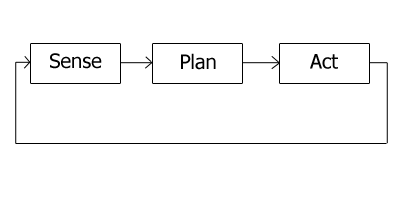
\includegraphics[width=1\columnwidth]{figs/Hierarchical.png}
\caption{Arquitetura hier�rquica tradicional.}
\label{hierarquica}
\end{figure}

De acordo com Marvin Minsky, uma m�quina (rob�) deveria tender a criar, por si
s�, um modelo abstrato do ambiente em que est� inserido (define-se
\emph{mundo}).
Caso fosse dado uma tarefa, ela primeiro poderia explorar solu��es dentro de seu modelo abstrato e, ent�o,
experiment�-las externamente. Seria como realizar uma simula��o interna
e, caso funcionasse, realiz�-la no mundo real.

\subsection{Rob�s deliberativos}
Entre 1966 e 1972, Charles Rosen e Nils Nisson da Universidade de Stanford
criaram o Shakey, primeiro rob� m�vel aut�nomo (figura~\ref{SHAKEY_1}). Foi
desenvolvida uma intelig�ncia artificial, \textit{problem solver}, chamada
STRIPS. Este sistema � um planejador de trajet�rias que armazena as imforma��es
do ambiente (mapas e obst�culos) de maneira simb�lica, e se dada uma tarefa de
deslocamento (\textit{goto}), � realizada uma busca l�gica pelo sistema. 

Em 1977, come�ou a ser desenvolvido o projeto HILARE (figura~\ref{hilare}), no
Laboratoire d'Automatique et d'Analyse des Syst�mes (LAAS), Toulouse, France.
O rob� possu�a sensores como c�mera, ultrassons e laser para medir
dist�ncia, sendo poss�vel atualizar o seu mundo com acur�cia. Seu mundo era
representado por modelos geom�tricos e um modelo relacional que expressava a
conectividade dos quartos e corredores (simb�lico) \cite{norelis1989control}.

Tamb�m em 1977, o Stanford Cart foi criado por Moravec para navega��o e desvio
de obst�culos \cite{moravec1977towards}. Os obst�culos eram identificados pelo
rob� durante a opera��o e representados em seu mundo interno como
esferas. O rob� possu�a uma segunda representa��o do mundo, simb�lica por
grafos.

Em 1969, Victor Scheinman, Universidade de Stanford
\cite{scheinman1969design}, inventou o primeiro manipulador rob�tico
totalmente el�trico de seis elos e com solu��o completa e integrada de
cinem�tica inversa. Isto �, dado um ponto qualquer pertencente ao espa�o de
trabalho do manipulador, este calcula o �ngulo das juntas de forma que o
efetuador alcance o ponto especificado. Isso permitiu que o manipulador
percorresse trajet�rias arbitr�rias. At� os dias atuais, 2015, � ampla a
utiliza��o de manipuladores industriais. A sofistica��o destes sistemas j�
possibilita que estes armazenem todo o conhecimento do mundo e executem tarefas
aut�nomas (figura~\ref{manipulador}).

\begin{figure}[h!]
\centering
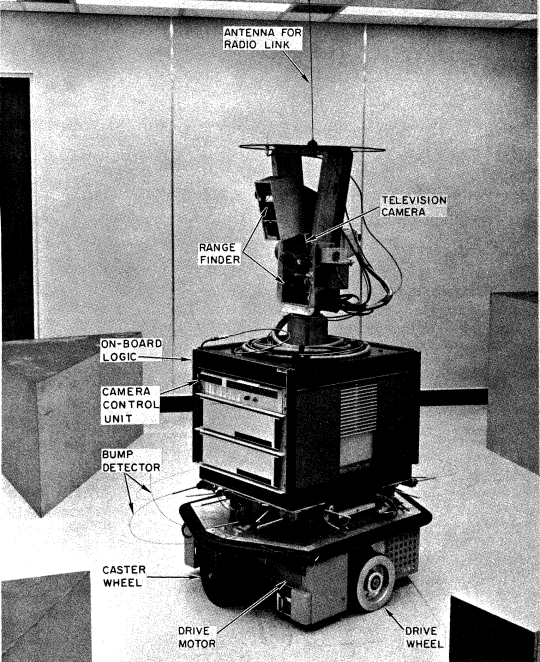
\includegraphics[width=1\columnwidth]{figs/SHAKEY_1.png}
\caption{Shakey robot}
\label{SHAKEY_1}
\end{figure}

\begin{figure}[h!]
\centering
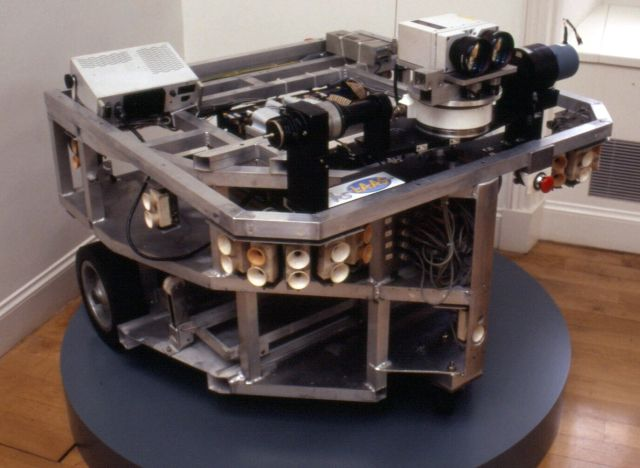
\includegraphics[width=1\columnwidth]{figs/HILARE.jpg}
\caption{HILARE}
\label{hilare}
\end{figure}

\begin{figure}[h!]
\centering
\includegraphics[width=1\columnwidth]{figs/MANIPULADOR.jpg}
\caption{Manipulador rob�tico atual}
\label{manipulador}
\end{figure}

%TODO: Verificar controle de miss�o dos modelos
\subsection{Arquiteturas deliberativas}
As arquiteturas deliberativas s�o sistemas hier�rquicos com a l�gica
\textit{SPA}. S�o utilizados em sistemas rob�ticos at� hoje, quando a aplica��o
favorece seu uso e o poder computacional n�o � uma restri��o.
Destacam-se os modelos de Albus, NASREM, \textit{Nested Hierarchical Controllers} e o \emph{Intelligent Mobile
Robot System}.

\subsubsection{Modelo de Albus}

Albus foi o pioneiro e mais influente autor de teorias em arquiteturas
deliberativas, \cite{albus1991outline}. Sua grande contribui��o foi a
formaliza��o e defini��o de diversos termos amplamente utilizados em automa��o e controle. Dentre outros, destaca-se o
teorema de que h� quatro sistemas que comp�em a intelig�ncia: processamento de
sensores, modelo do mundo, gera��o de comportamentos e julgamento de valor. As
entradas desses elementos s�o os sensores e suas sa�das s�o os atuadores:

\begin{itemize}
  \item Atuadores: as sa�das de um sistema inteligente pe produzida por
  atuadores, como mover, posicionar bra�os, pernas, m�os, olhos e etc. Os
  atuadores naturais s�o os m�sculos e as gl�ndulas, j� os atuadores de m�quinas
  s�o motores, pist�es e v�lvulas.
  \item Sensores: s�o as entradas de um sistema inteligente, como sensores de
  for�a, torque, posi��o, velocidade, vibra��o, ac�stico, gases, temperatura e
  muitos outros. Monitoram o mundo e o estado interno do sistema, e prov� dados
  ao sistema de processamento sensorial.
  \item Processamento sensorial: sistema que compara novas observa��es com a
  expectativa interna do modelo do mundo. Integra e armazena as diferen�as e
  semelhan�as encontradas, a fim de reconhecer padr�es, objetos e rela��es no
  mundo.
  \item Modelo do mundo: � a melhor estimativa que o sistema inteligente possui
  do mundo, e atualizado pelo processamento sensorial. � um banco de dados com
  todo o conhecimento do mundo e cont�m uma capacidade de simula��o que gera expectativas e predi��es. O modelo do mundo
  pode prover informa��es do passado, presente e prev� estados futuros.
  Os dados s�o importantes para: o gerador de comportamentos escolher o plano
  adequado para execu��o das a��es; o processamento sensorial fazer correla��es,
  compara��o de modelos, e reconhecimento de objetos, estados e eventos; e o
  sistema de julgamento de valor computar valores de custo, benef�cio, risco,
  incerteza, import�ncia e outros.
  \item Julgamento de valor: este � o sistema que determina o que � bom ou ruim,
  importante ou trivial, certo ou improv�vel. Computa custos, riscos e
  benef�cios de situa��es observadas e atividades planejadas.
  \item Gerador de comportamentos: elemento que seleciona objetivos e planos,
  executa e monitora a��es, e modifica planos existentes quando alguma situa��o
  do mundo exigir. Tarefas s�o decompostas em subtarefas, e subtarefas s�o
  sequ�ncias de objetivos. A ordem l�gica de funcionamento �: o gerador de
  comportamentos cria planos, o modelo do mundo predita o resultado do plano, e
  o julgamento de valor avalia os resultados. O gerador de comportamento
  seleciona o plano com a avalia��o mais alta.
\end{itemize}

As rela��es entre os elementos do sistema inteligente est�o representados na
figura~\ref{albus}.  Esses elementos e suas rela��es possibilitaram a cria��o de
diversas arquiteturas.

\begin{figure}[h!]
\centering
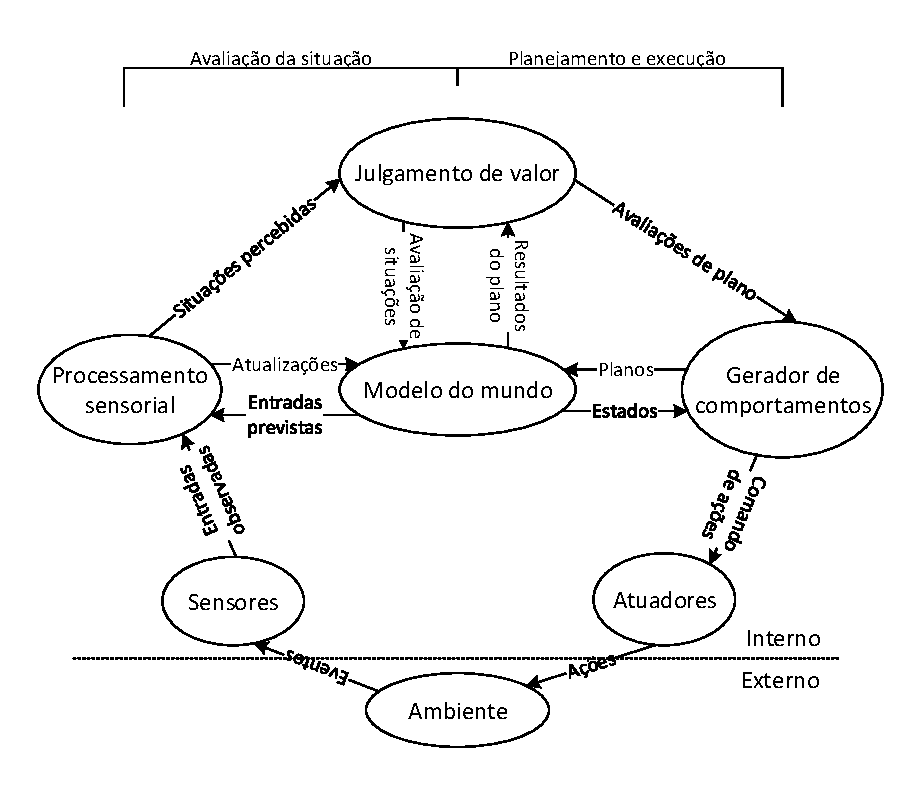
\includegraphics[width=1\columnwidth]{figs/albus.pdf}
\caption{Arquitetura de Albus para sistemas deliberativos.}
\label{albus}
\end{figure}

Vale ressaltar que, nesta arquitetura, o \textit{gerador de comportamentos} faz
o papel de controlador de miss�o.

\subsubsection{NASREM}
O NASREM \cite{albus1989nasa} foi uma arquitetura utilizada pela
NASA e possu�a uma arquitetura com seis n�veis de
funcionalidade (figura~\ref{nasrem}):

\begin{enumerate}
  \item Servo: prov� o controle dos atuadores do rob� (posi��o, velocidade e
  etc).
  \item Primitiva: determina as primitivas de movimento para gerar trajet�rias
  suaves.
  \item Movimento elementar: define e planeja trajet�rias livre de colis�es.
  \item Tarefa: converte a��es desejadas de um objeto em sequ�ncias de
  movimentos elementares.
  \item Compartimento de servi�os: converte a��es de grupos de objetos em
  tarefas de um objeto.
  \item Miss�o: decomp�e o plano de miss�o em alto n�vel em compartimento de
  servi�os.
\end{enumerate}

Vale ressaltar que, no modelo NASREM, o operador tem acesso a qualquer n�vel
hier�rquico do rob� e pode tomar o controle do rob� para si, al�m de poder
substituir as entradas de sensores, modelo do mundo e outros. Dessa forma, o
n�vel de autonomia do rob� pode ser desenvolvido de forma incremental.

A arquitetura hier�rquica proposta em NASREM permite modularidade e prop�e uma
metodologia de software.  
 
\begin{figure}[h!]
\centering
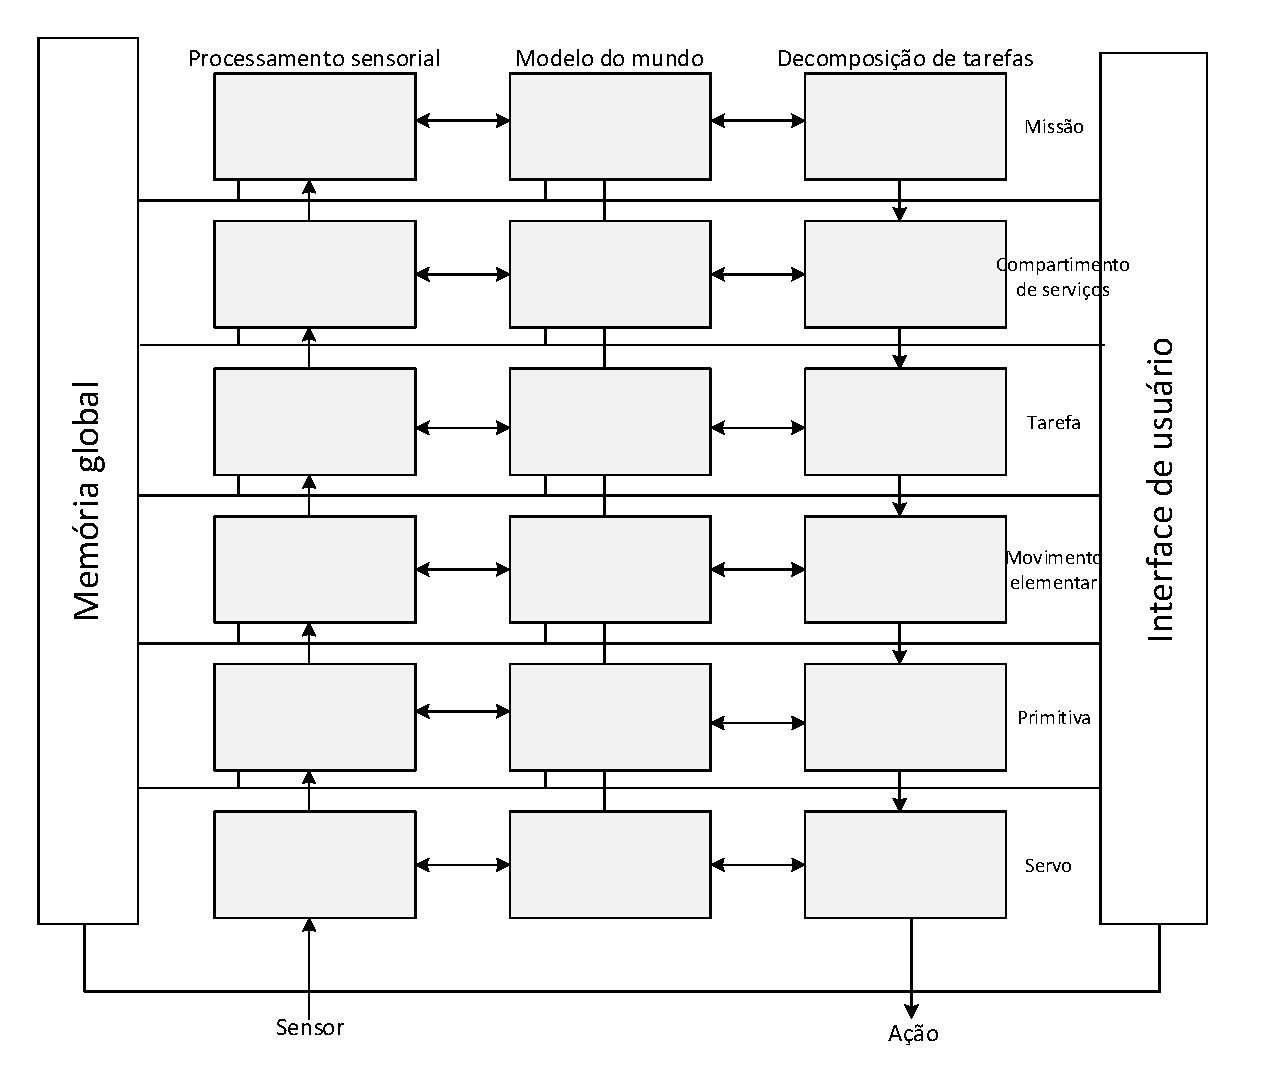
\includegraphics[width=1\columnwidth]{figs/NASREM.pdf}
\caption{Arquitetura NASREM.}
\label{nasrem}
\end{figure}

\subsubsection{\textit{Nested Hierarchical Controllers}}
O \textit{Nested Hierarchical Controllers} (NHC) consiste tamb�m em seis
n�veis hier�rquicos: planejador da miss�o, navegador, piloto, monitor de
trajet�ria, controlador, e sistema de controle de baixo n�vel. H� tamb�m
constante atualiza��o do modelo do mundo por um sistema de sensoriamento.

O planejamento � decomposto em planejador da miss�o, navegador e piloto e seus
m�dulos s�o executados sequencialmente, tornando-se mais espec�fico e detalhado.
A l�gica � hier�rquica: o planejador de miss�o envia trechos da miss�o para o
navegador, o qual envia trechos de trajet�ria para o piloto, que determina a��es
ao controlador de baixo n�vel. A utiliza��o do mapa interno do rob� por cada
m�dulo � diferente, enquanto o planejador usa o mapa global, o piloto recebe
informa��es locais. Vale observar que, quando o modelo do mundo � atualizado,
muitas vezes n�o h� necessidade de o planejador atualizar toda a miss�o e
recome�ar o ciclo de planejamento, apenas o piloto pode recalcular a trajet�ria
local. 
%TODO: FIGURA 

\subsubsection{\textit{Intelligent Mobile Robot System}}
Em 1991, Saridis \cite{wang1991petri} cria o \emph{Intelligent Mobile
Robot System} (IMRS) baseado na teoria de intelig�ncia hier�rquica de controle
\cite{saridis1988analytical}. Saridis utiliza redes de Petri como m�dulos
b�sicos da arquitetura para traduzir os comandos gerados pelo n�vel de
organiza��o em algo compreens�vel para o n�vel de execu��o.

O IMRS possui a seguinte arquitetura (figura~\ref{Saridis_1}):
\begin{itemize}
  \item N�vel organizacional (organizador de tarefas): gera tarefas de
  movimenta��o de alto n�vel.
  \item N�vel de coordena��o: funciona como uma interface entre o n�vel
  organizacional e o de execu��o. O n�vel � composto por um remetente e alguns
  coordenadores. O remetente recebe o plano da tarefa do organizador, decomp�e a
  tarefa em a��es de controle e remete aos coordenadores. Os coordenadores
  traduzem os comandos de controle em instru��es de opera��o e transmite ao
  n�vel de execu��o.
  \item N�vel de execu��o: executa a instru��o proveniente do n�vel de
  coordena��o e reporta seus resultados a ele.
\end{itemize}

O n�vel de coordena��o do IMRS � composto por um remetente
(\emph{Dispatcher}) e tr�s coordenadores: sistema de vis�o (VS), desvio de
obst�culo e controle de rastreamento (OATC), e planejamento de trajet�rias (PP).
Com o modelo de redes de Petri n�o � poss�vel implementar o esquema de linguagem de
decis�o para descrever a tradu��o de tarefas entre remetente e coordenadores.
Portanto, os \emph{Petri Net Transducers} (PNTs) foram introduzidos como
tradutores de linguagem (protocolo): $PNT = (N,\Sigma,
\Delta, \sigma, \mu, F)$. Onde:
\begin{itemize}
	\item A rede de Petri $N=(P,T,I,O)$, $P$ lugares, $T$
transi��es, fun��o de entrada $I$, fun��o de sa�da $O$, � o controle da
tradu��o;
	\item $\mu$ � o estado inicial de $N$;
	\item $\Sigma$ � o alfabeto de entrada, representa tarefas de entradas;
	\item $\Delta$ � o alfabeto de sa�da, representa tarefas de sa�da; 
	\item $\sigma$ especifica, para uma dada tarefa de entrada, as transi��es em
$N$ e as subtarefas de sa�da que podem ser usadas na tarefa;
	\item $F$ � o estado final. Indica o fim da tradu��o da tarefa;
\end{itemize}    

Os quatro PNT's s�o combinados para realizarem a tradu��o de tarefas no N�vel
de Coordena��o: remetente, sistema de vis�o, desvio de obst�culo
e controle de rastreamento, e planejamento de trajet�rias. A
figura~\ref{Saridis_2} mostra o modelo de rede de Petri para o Remetente.
%Ser� brevemente descrito o componente Remetente (\emph{Dispatcher}) do modelo
% de N�vel de Coordena��o para melhor entendimento do PNT.

%Foram definidas quatro tarefas para o N�vel de Coordena��o: 1) \emph{wmu}:
%atualiza��o da mem�ria 3-D do ambiente; 2) \emph{mod}: detec��o de objetos em
%movimento; 3) \emph{pp}: planejamento de trajet�rias; 4) \emph{moac}: desvio de
%obst�culos e controle de rastreamento. A figura~\ref{Saridis_2} mostra o modelo
%de rede de Petri para o Remetente.

\begin{figure}[h!]
\centering
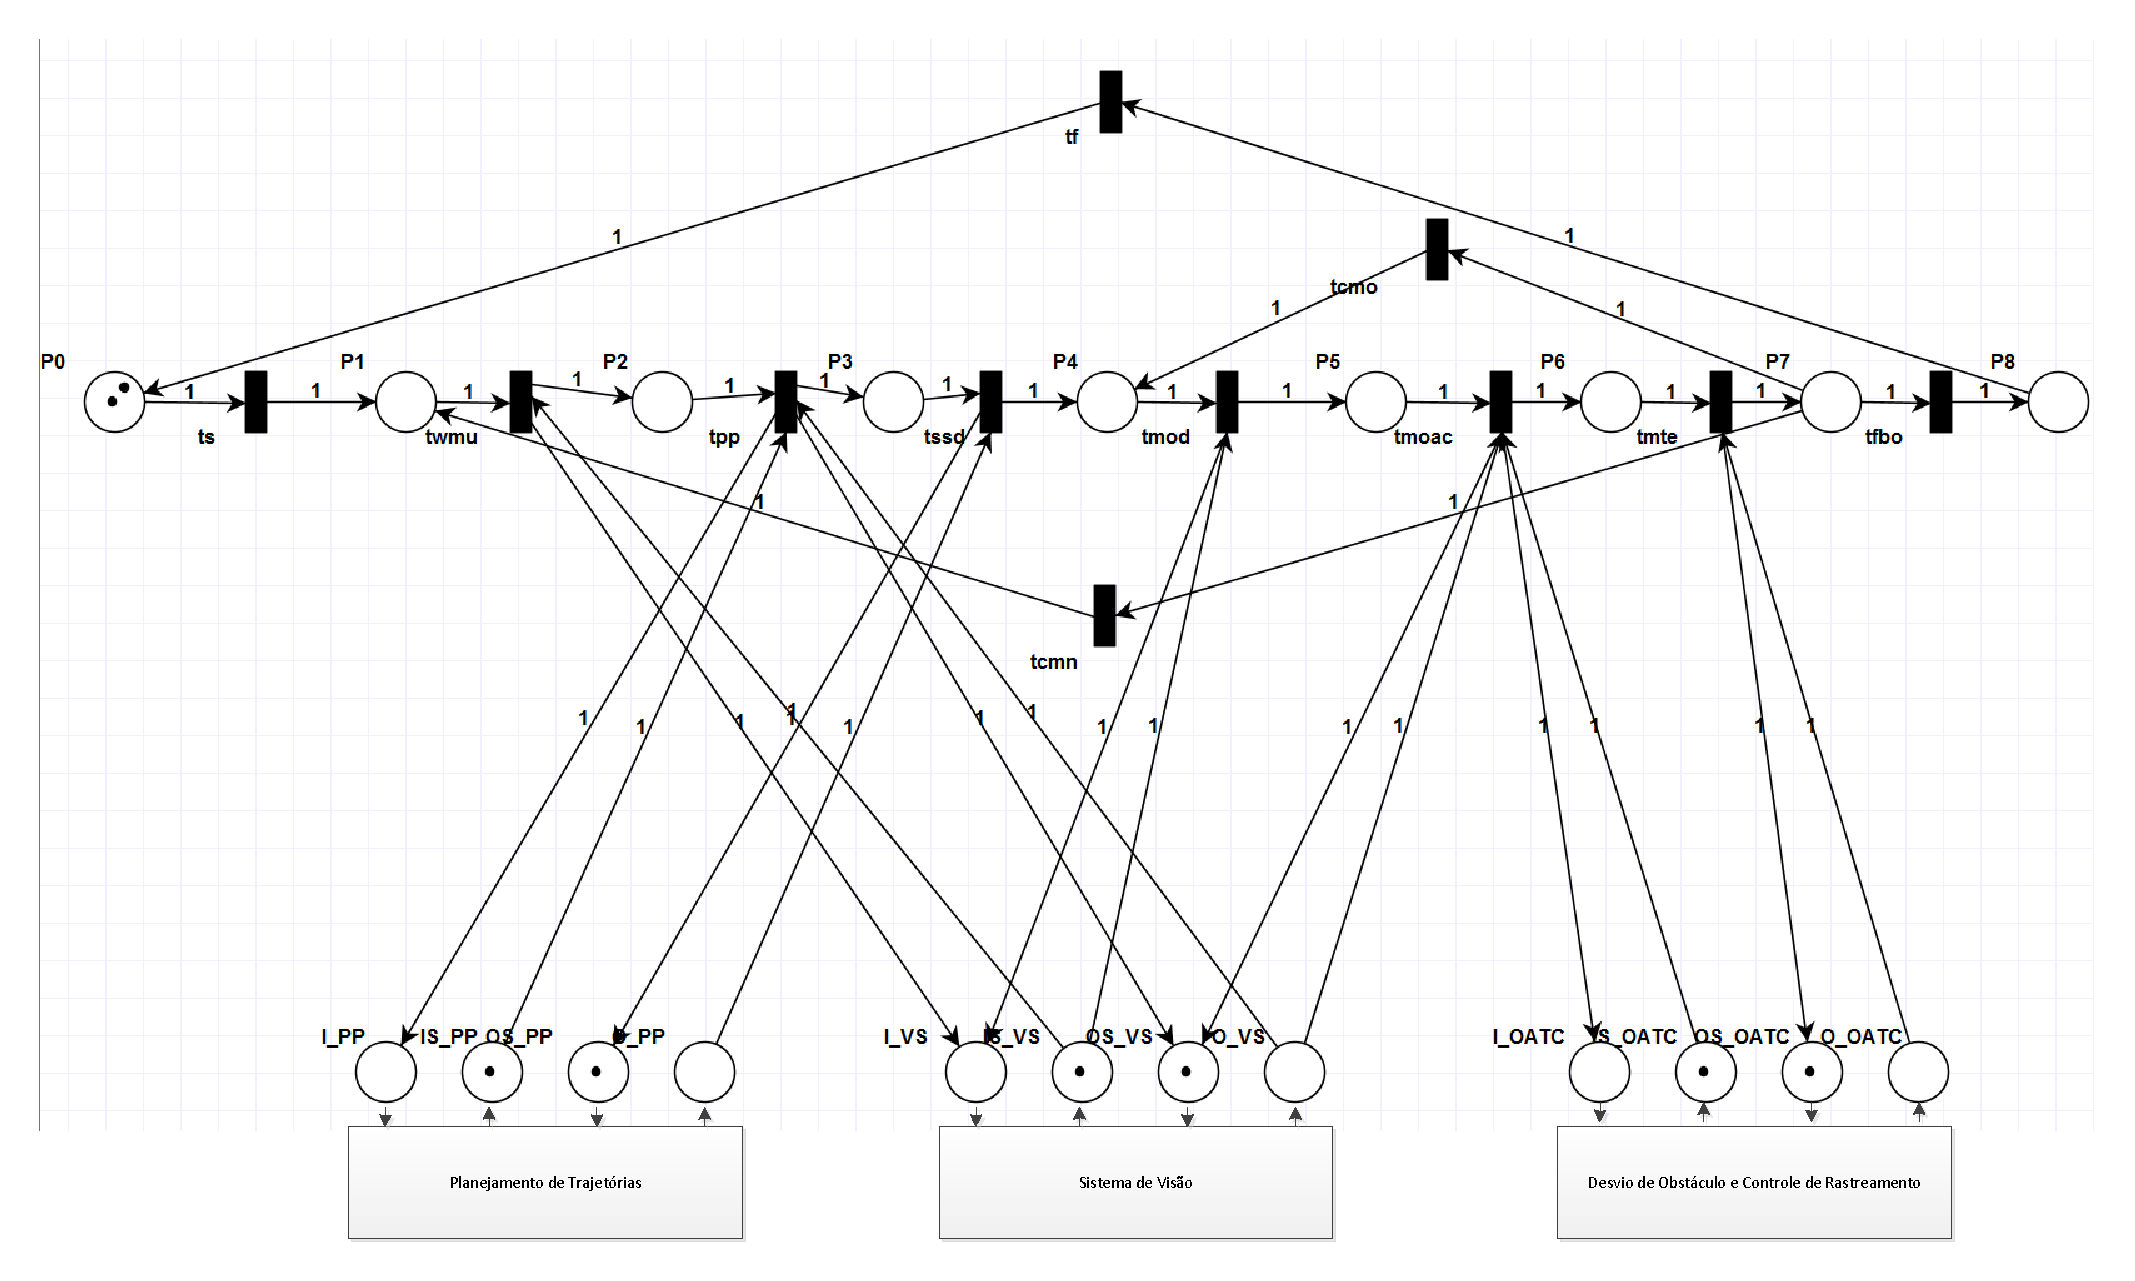
\includegraphics[width=1\columnwidth,angle=90]{figs/SARIDIS_2.pdf}
\caption{Estrutura do n�vel de coordena��o com foco na rede de Petri do
Remetente}
\label{Saridis_2}
\end{figure}

A modelagem do sistema utilizando redes de Petri proporcionaram, como pode ser
visto na figura~\ref{Saridis_2}, algumas funcionalidades essenciais em uma
arquitetura rob�tica: a capacidade de executar duas tarefas simultaneamente, por
exemplo, movimenta��o e planejamento de trajet�rias; e o \emph{Input Semaphore},
que impede um processo de ser executado at� outro ser finalizado.
  
Saridis salienta os benef�cios das PNT:
\begin{itemize}
  \item Redes de Petri podem ser usadas como m�dulos b�sicos para sistemas de
  controle de miss�o de rob�s m�veis.
  \item A comunica��o e conex�o de m�dulos s�o eficientes entre redes de Petri.
  \item Controle e mecanismo de comunica��o para coordena��o de tarefas de um
  rob� m�vel podem ser realizados com redes de Petri.
\end{itemize} 

A arquitetura de Saridis � uma contribui��o importante por criar um n�vel
organizacional, separando o n�vel do desenvolvedor de baixo n�vel e um
n�vel de alto n�vel para um operador (usu�rio). Al�m disso, as redes de Petri
assumem um importante papel como m�dulo b�sico de controle para seu sistema
IMRS. As redes de Petri foram originalmente introduzidas para descrever as
comunica��es de m�quinas de estado finito (FSM), possibilitando flexibilidade
e robustez, e � provado que redes de Petri s�o uma excelente ferramenta para
modelagem de sistemas, sobretudo quando envolvem tarefas conflitantes ou
simult�neas \cite{murata1989petri}.


\subsection{An�lise cr�tica}
A abordagem deliberativa simula, de certa forma, o processo de planejamento e
tomada de decis�o do ser humano. H� um n�cleo (c�rebro) que
processa todos os dados sensorias e armazena o mundo, isto �, o ambiente em que
o rob� est� inserido, de maneira simb�lica, geom�trica ou outros tipos de
mapeamento. Al�m disso, o n�cleo planeja todas as a��es para uma determinada
tarefa, consultando sua ideia de mundo intensivamente. H�, tamb�m, sensores que
enviam suas novas informa��es periodicamente para o n�cleo, (�rg�os receptivos:
vis�o, olfato, e etc), atualizando o mundo. E h� atuadores (m�sculos)
necess�rios para a realiza��o das tarefas (figura~\ref{brain}).

� f�cil observar que a arquitetura deliberativa � dependente do
modelo de mundo armazenado e suas atualiza��es peri�dicas. Portanto, a
utiliza��o da abordagem deliberativa em ambientes extremamente din�micos pode ser muito
custosa devido �s atualiza��es e ao replanejamento. Al�m disso, � f�cil observar
que a arquitetura SPA dificulta a cria��o de sistemas em tempo real eficientes.
Dessa forma, rob�s m�veis em ambientes muito din�micos, como o carro aut�nomo da
google (figura~\ref{googlecar}), n�o s�o aplica��es favor�veis para esta
arquitetura.

\begin{figure}[h!]
\centering
\includegraphics[width=1\columnwidth]{figs/BRAIN.png}
\caption{Comparativo da arquitetura deliberativa com o ser humano.}
\label{brain}
\end{figure}

\begin{figure}[h!]
\centering
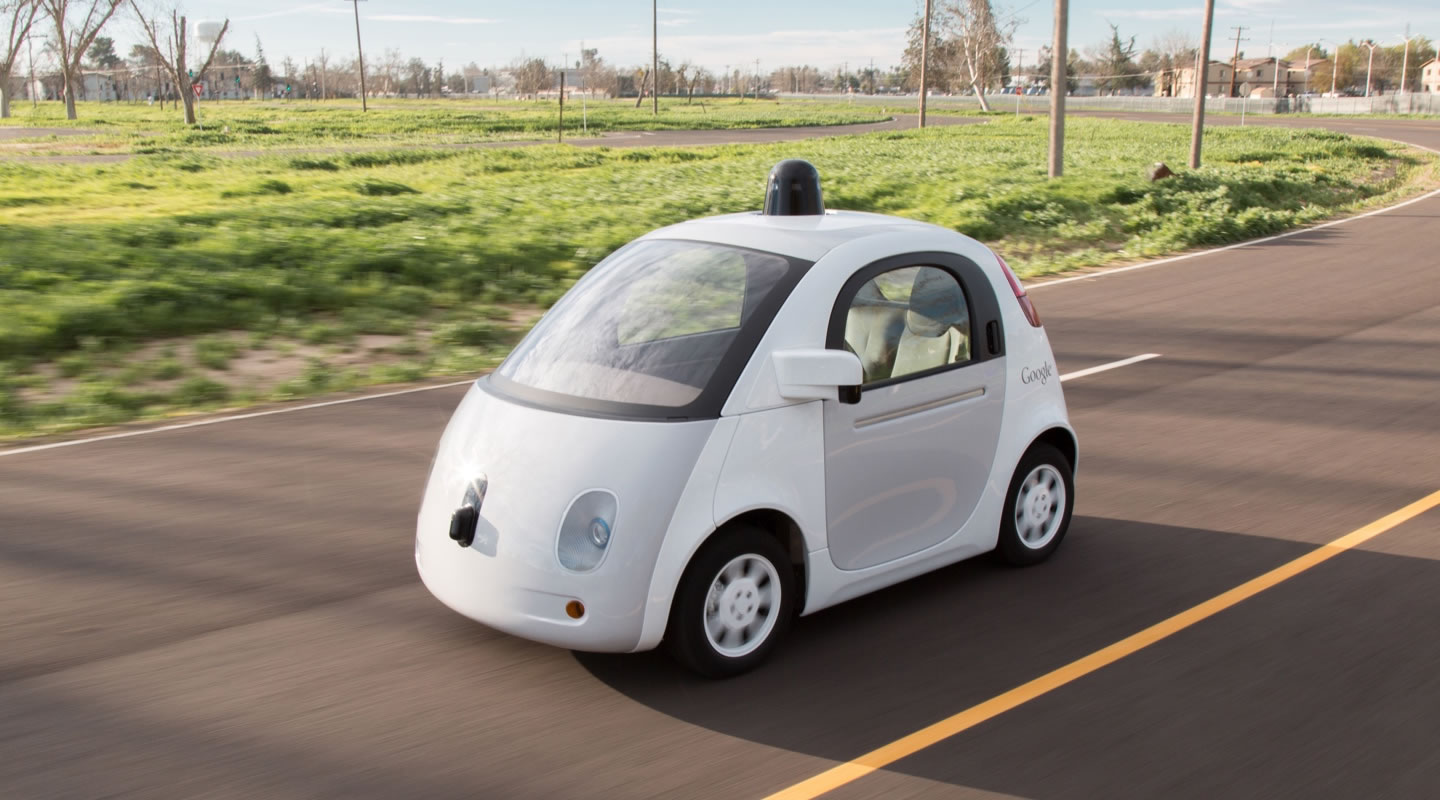
\includegraphics[width=1\columnwidth]{figs/googlecar.jpg}
\caption{Projeto da google 2011- para o desenvolvimento de um carro aut�nomo.}
\label{googlecar}
\end{figure}

\section{Paradigma reativo}

Sistemas de arquitetura reativa tamb�m s�o chamados de sistemas baseados em
comportamentos. Os rob�s s�o programados para agir atrav�s de ativa��o de uma
cole��o de comportamentos primitivos de baixo n�vel. De acordo com
\cite{arkin1995reactive}, as principais caracter�sticas de sistemas puramente
reativos s�o:

\begin{itemize}
  \item Comportamentos s�o como elementos construtivos: s�o um par sensor-motor,
  onde o sensor prov� informa��o necess�ria para o motor executar uma a��o
  reativa, como desvio de obst�culo, atrair-se a objetivos, escapar de
  predadores e etc.
  \item N�o h� cria��o ou manuten��o precisa do modelo do mundo. Os sistemas
  reagem ao est�mulo do mundo, extremamente �til para mundos din�micos e
  hostis.
  \item Comportamentos de animais s�o normalmente utilizados para modelar esses
  sistemas.
\end{itemize}

Dessa forma, controle reativo � uma t�cnica que une percep��o e a��o,
tipicamente no contexto de comportamentos motores, para produzir respostas
rob�ticas em tempo real em mundos din�micos e n�o estruturados.

Em 1986, um dos primeiros estudos em sistemas reativos foi desenvolvido por
Rodney Brooks \cite{brooks1986robust}. Este estudo � a base para diversos
trabalhos atuais que envolvem rob�s reativos m�veis. Os desafios de
rob�s aut�nomos apontados por Brooks e que ainda ilustram os problemas da
atualidade s�o: \emph{m�ltiplos objetivos}, \emph{m�ltiplos sensores},
\emph{robustez} e \emph{extensibilidade}. De acordo com Brooks, esses desafios
n�o s�o suportados pela arquitetura tradicional (paradigma hier�rquico) de um
sistema de controle.

Os m�ltiplos objetivos de rob�s m�veis podem:
\begin{itemize}
  \item Ser conflitantes: por exemplo, um rob� pode estar tentando alcan�ar um
  determinado ponto no espa�o, por�m evitando obst�culos locais.
  \item Ter rela��es de prioridade: por exemplo, um rob� que inspeciona trilhos
  de tr�m deve sair dos trilhos ao ouvir o sinal de um tr�m chegando, mesmo se estiver
  finalizando a opera��o.
  \item Ser denpendentes: objetivos de \emph{alto n�vel} englobam diversos
  objetivos de \emph{baixo n�vel}. No caso do exemplo acima, o rob� que sai do
  trilho para evitar o tr�m deve se manter equilibrado para n�o cair. Artigos
  recentes, como em \cite{fryxell1996navigation} separam esses objetivos em
  \emph{tarefas} (objetivos de \emph{alto n�vel}) e \emph{primitivas do ve�culo}.
\end{itemize}

Rob�s s�o normalmente providos de m�ltiplos sensores e suas diversas
informa��es podem ser redundantes, conflitantes ou complementares,
podendo ser utilizadas para uma mesma tarefa do rob�.
Por exemplo, encoders para odometria e c�meras fixas ao rob�
podem ser utilizados para localiza��o, de forma que se complementem.
Os sensores podem apresentar erros ou resultados conflitantes, portanto a fus�o
da informa��o de m�ltiplos sensores, a determina��o de seus graus de
confiabilidade e em quais tarefas devem ser considerados s�o decis�es que o
rob� deve saber fazer.

Um rob� deve ser robusto, isto �, em caso de falha de um sensor, o rob�
deve se adaptar e utilizar os outros sensores que ainda funcionam para realizar as
tarefas. Ou em caso de altera��es no ambiente, o rob� deve ser
capaz de cumprir determinadas fun��es essenciais.

A extensibilidade constitui em acrescentar mais sensores e,
portanto, aumentar a capacidade do rob�, sendo poss�vel a execu��o de novas
tarefas. Por�m, esta afirma��o � normalmente criticada por alguns autores j� que
existe um limite imposto pelo processamento do rob�, j� que um novo hardware
(sensor) � adicionado, mas o processamento (computador) n�o � substitu�do e sua
capacidade n�o � aumentada.

Brooks prop�e um dos primeiros sistemas baseados em comportamentos, uma
arquitetura que tem como objetivo descentralizar a tomada de decis�o de um
modelo central, como pode ser visto na figura~\ref{BROOKS_1}. O autor comenta
que essa decomposi��o conduz a uma arquitetura radicalmente diferente para
sistema de controle de rob�s m�veis em estrat�gias de implementa��o a n�vel de
hardware e com grandes vantagens em robustez, desenvolvimento e teste.

\begin{figure}[h!]
\centering
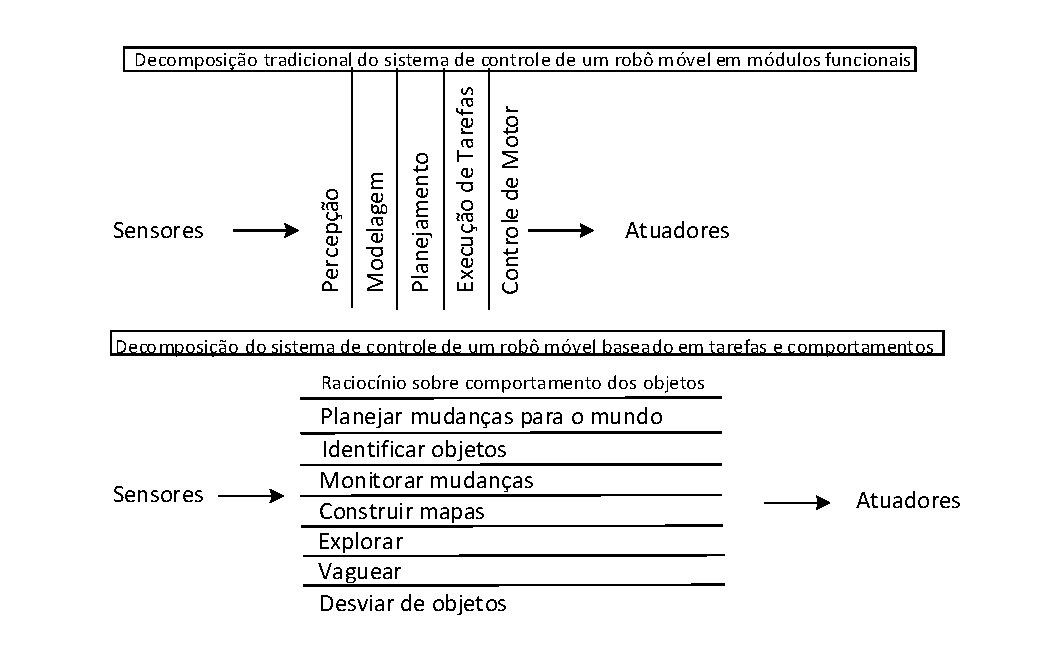
\includegraphics[width=1\columnwidth]{figs/BROOKS_1.pdf}
\caption{Arquitetura para sistema de controle de rob�s m�veis por Brooks}
\label{BROOKS_1}
\end{figure}

\subsection{Rob�s reativos}
Antes mesmo de Brooks, ou seja, antes da formaliza��o de toda a teoria em
sistemas reativos, simples rob�s eram criados na l�gica de controle reativo e de
comportamentos. Em 1953, por exemplo, Grey Walter \cite{holland1997grey}
desenvolveu uma ``tartaruga'' el�trica capaz de se movimentar pelo ambiente,
evitando luz intensa (``amea�as'') e atra�da por certos objetivos. Vale
observar a caracter�stica de perceber baixo n�vel de bateria e procurar
uma esta��o de recarga, comportamento que se sobrep�e aos outros. Os
comportamentos s�o simples e n�o h� representa��o abstrata do mundo:
dirigir-se para luz fraca; fugir de luz forte; e evitar obst�culos.

Em 1984, ve�culos simples e puramente reativos com os pares cl�ssicos
sensor-motor foram desenvolvidos pelo psicologista Braitenberg
\cite{braitenberg1986vehicles}, a fim de simular sentimentos, como covardia,
agressividade e outros. 

Em 2002 at� os dias atuais, o rob� iRobot Roomba ganha destaque comercial e
executa uma simples tarefa dom�stica: limpar o ch�o. Em sua arquitetura, o rob�
Roomba possui apenas algumas fun��es reativas, como esquivar-se e locomover-se,
e, em suas vers�es antigas, foi constatado que n�o possui o modelo do mundo,
mapa, dentro de si \cite{tribelhorn2007evaluating}.

%TODO: Verificar controle de miss�o dos modelos
\subsection{Arquiteturas reativas}
As arquiteturas reativas foram formalmente introduzidas em 1986 por
Roodney Brooks. O roboticista, futuro fundador da empresa iRobot, vivenciou uma
�poca de processadores lentos e de alto custo, dificultando o uso de diversos
sensores e a armazenagem do modelo do mundo no rob�. Simula��es de tarefas,
atualiza��es do mundo e an�lise de sensores como c�meras eram extremamente
complexas para rob�s e imposs�veis de serem executadas em tempo real. Brooks
vislumbrou como solu��o o processamento paralelo, evitar o uso de um modelo do
mundo e criar m�dulos puramente reativos, pares sensor-motor, que juntos comp�em
o rob�. 

O sistema de controle de arquiteturas reativas utilizam informa��es locais
do meio, obtidas pelos sensores do rob�. Estas s�o simplificadamente tratadas,
de forma que a a��o ao est�mulo � tomada rapidamente e, assim, os rob�s reativos
podem responder de forma mais r�pida a varia��es do ambiente. A arquitetura
define como a informa��o � mapeada em uma a��o e como � feita a coordena��o dos
pares est�mulo-a��o (comportamentos reativos).

De acordo com Arkin \cite{arkin1998behavior}, h� duas classes predominantes
para a fun��o de coordena��o: competitiva e cooperativa.

Um conflito ocorre quando dois ou mais comportamentos est�o ativos ao mesmo
tempo e possuem respostas diferentes. Nesse caso, a coordena��o de forma
competitiva entra em a��o, escolhendo um dos comportamentos para a a��o final do
rob�. A prioridade de um comportamento sobre os demais pode ser definida
explicitamente em uma hierarquia entre os comportamentos, ou pode haver uma
vota��o por uma a��o, ou outros m�todos. O exemplo de sistema reativo com
coordena��o do tipo competitiva � o desenvolvido por Brooks, arquitetura de
subsun��o.

Na arquitetura cooperativa, a a��o do rob� � a fus�o da resposta de todos os
comportamentos ativos. A arquitetura reativa esquema motor de Arkin � um exemplo
claro deste tipo de coordena��o, onde cada comportamento influencia o movimento
do rob� por meio de um vetor de for�a artificial e a a��o resultante �
determinada pela soma vetoria de todos os vetores de for�a.


\subsubsection{Arquitetura de subsun��o}
A arquitetura de subsun��o �, neste trabalho, destacada, exemplificada e
minuciosamente comentada, j� que sua l�gica ser� o cerne da implementa��o da
camada reativa da DORIS.

Na figura~\ref{BROOKS_1}, Brooks define \emph{N�veis de compet�ncia}, que s�o
classes de comportamentos desejados para o rob� sobre todos os ambientes que ele
pode encontrar. As classes definidas por Brooks s�o:
\begin{enumerate}
\setcounter{enumi}{-1}
  \item Evitar contato com objetos (estacion�rios ou m�veis);
  \item Vaguear sem rumo e sem bater em objetos;
  \item Explorar o ambiente utilizando sensores, definir lugares alcan��veis, e
  seguir rumo em suas dire��es;
  \item Construir um mini-mapa do ambiente e planejar trajet�rias de um lugar
  para outro;
  \item Observar mudan�as no ambiente;
  \item Raciocinar sobre o ambiente em termos de objetos identific�veis e
  realizar tarefas relacionadas a certos objetos;
  \item Formular e executar planos que envolvam mudar o estado do ambiente como
  desejado;
  \item Raciocinar sobre o comportamento de objetos no ambiente e modificar
  planos quando necess�rio;
\end{enumerate}

Cada n�vel de compet�ncia inclui, como subconjunto, os
n�veis de compet�ncia anteriores.

Ap�s a decomposi��o na nova arquitetura, Brooks define as \emph{Camadas de
Controle}, correspondentes a cada n�vel de compet�ncia. A ideia dessa abordagem
� adicionar camadas de controle a n�veis de compet�ncias superiores sem precisar
alterar a camada do n�vel inferior. Inicia-se, portanto, com a camada de
controle para o n�vel zero de compet�ncia, esta ser� testada e n�o mais
alterada. Ap�s, � criada a camanda de n�vel 1, capaz de examinar os dados
da camada de n�vel 0 e injetar dados nas interfaces internas deste n�vel,
suprimindo seu tr�nsito de dados, figura~\ref{BROOKS_2}.

\begin{figure}[h!]
\centering
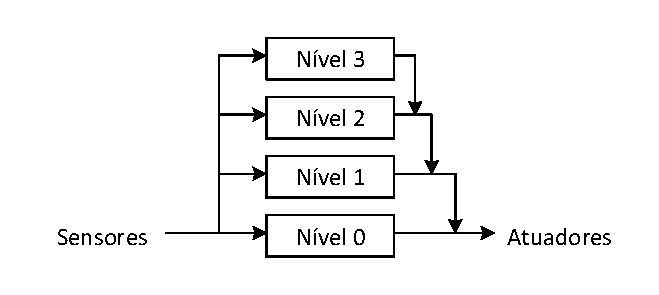
\includegraphics[width=1\columnwidth]{figs/BROOKS_2.pdf}
\caption{Camadas de controle de Brooks}
\label{BROOKS_2}
\end{figure}

A camada de controle n�vel zero deve garantir que o rob� n�o entre em contato
com outros objetos, estacion�rios ou m�veis. Portanto, o rob� deve desviar de
objetos que se aproximam ou parar se houver um objeto fixo em sua trajet�ria. A camada de controle n�vel 1, combinada a camada de controle n�vel 0, permite
 que o rob� vagueie sem colis�es. A figura~\ref{BROOKS_4} mostra o sistema de
 controle aumentado pelo n�vel da camada 1.


% \begin{figure}[h]
% \centering
% 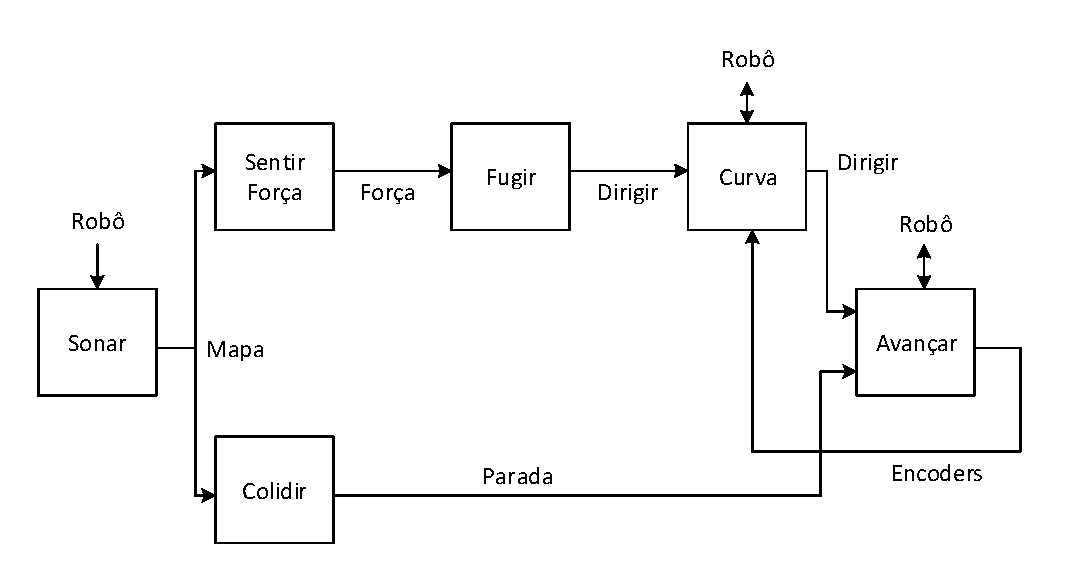
\includegraphics[width=1\columnwidth]{figs/BROOKS_3.pdf}
% \caption{N�vel 0 de controle do sistema}
% \label{BROOKS_3}
% \end{figure}
% 
% Segue pequena descri��o de cada m�dulo:
% \begin{itemize}
%   \item M�dulo \emph{Curva}: comunica-se diretamente com o rob� (atuadores).
%   Recebe uma mensagem \emph{Dirigir} especificando um �ngulo de giro seguido por
%   uma mensagem do m�dulo \emph{Avan�o} com uma determinada magnitude. Isso faz
%   com que o rob� realize uma curva e v� para o estado de \emph{Avan�o}.
%   \item M�dulo \emph{Avan�o}: comando faz rob� se movimentar (atuadores), mas
%   p�ra o rob� se receber mensagem do m�dulo \emph{Colis�o}. O rob� fica inativo
%   e mensagens do encoder � enviado ao m�dulo \emph{Curva}, funcionando como um
%   \emph{reset}, e podendo receber novos comandos.
%   \item M�dulo \emph{Sonar}: recebe um vetor de informa��es de sensores do rob�,
%   filtra os dados e produz um mapeamento de obst�culos para o rob� em
%   coordenadas polares.
%   \item M�dulo \emph{Colis�o}: monitora o mapa gerado pelo m�dulo \emph{Sonar}
%   e, se detectar um obst�culo, envia um sinal de parada. Observe que este m�dulo
%   funciona independentemente se o rob� est� em movimento ou parado.
%   \item M�dulo \emph{Sentir For�a}: cada obst�culo detectado � somado
%   como uma for�a repulsiva, gerando uma for�a resultante.
%   \item M�dulo \emph{Fugir}: monitora a for�a produzida pelos obst�culos e envia
%   comandos para o m�dulo \emph{Curva} se a for�a for significante.
% \end{itemize}
 
 

\begin{figure}[h!]
\centering
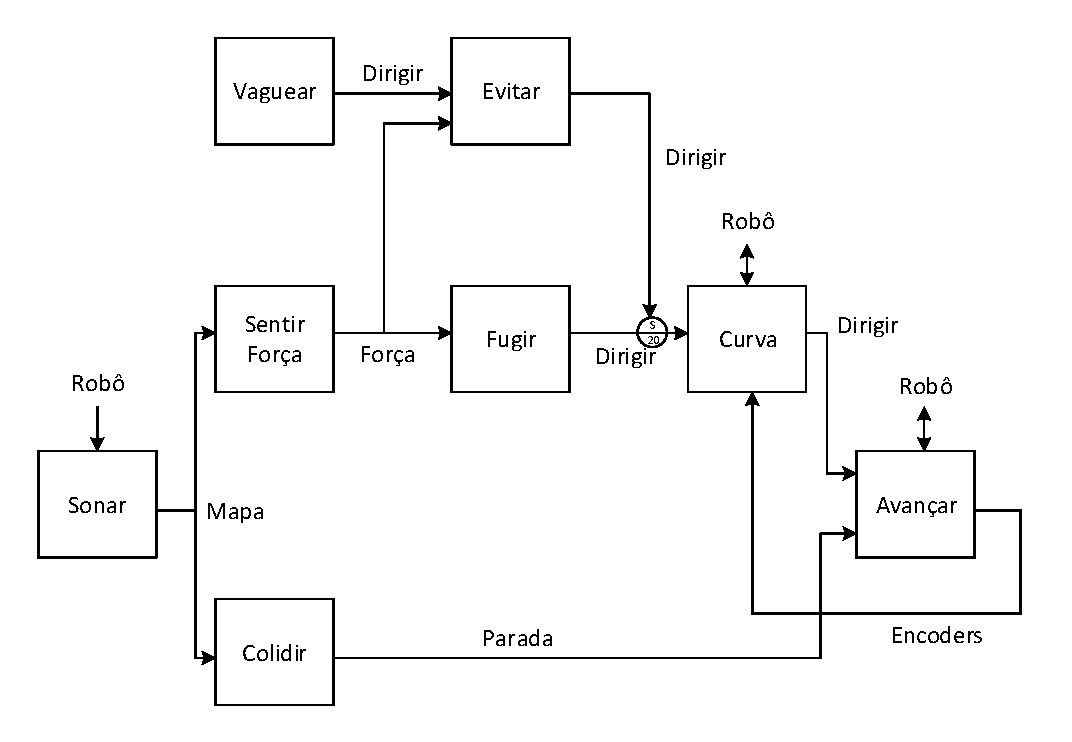
\includegraphics[width=1\columnwidth]{figs/BROOKS_4.pdf}
\caption{N�vel 0 e 1 de controle do sistema}
\label{BROOKS_4}
\end{figure}

% Segue pequena descri��o de cada m�dulo do n�vel 1:
% \begin{itemize}
%   \item M�dulo \emph{Vaguear}: gera nova dire��o para o rob� a cada 20 segundos.
%   \item M�dulo \emph{Evitar}: recebe resultado da for�a computada pelo n�vel 0
%   de controle e combina com a dire��o desejada pelo m�dulo \emph{Vaguear},
%   produzindo uma nova dire��o desejada sem obst�culos. Esse resultado presume as
%   computa��es do m�dulo \emph{Fugir}. Vale observar que o m�dulo \emph{Evitar}
%   suprime a sa�da do m�dulo \emph{Fugir} (mecanismo de supress�o). 
% \end{itemize}
% 
% Os problemas anteriormente da arquitetura hier�rquica apontados por Brooks
% s�o solucionados pela nova arquitetura:
% \begin{itemize}
%   \item M�ltiplos objetivos: camadas individuais podem trabalhar em objetivos
%   individuais ao mesmo tempo. Os n�veis das camadas de controle e o mecanismo de
%   supress�o do tr�nsito de dados resolvem os problemas de conflito, depend�ncia
%   e prioridade;
%   \item M�ltiplos sensores: as camadas utilizam os dados dos sensores
%   independentemente, de forma que n�o h� necessidade de se preocupar com a
%   fus�o;
%   \item Robustez: al�m do uso inteligente de sensores, camadas de controle de
%   n�vel inferior continuam a funcionar quando novas camadas de n�vel superior
%   s�o adicionadas;
%   \item Extensibilidade: cada camada de controle pode possuir o seu pr�prio
%   processador, resolvendo o problema de adicionar sensores indefinidamente e
%   consumir o processamento;
% \end{itemize}

A estrutura das camadas de controle foram constru�das por um conjunto de
pequenos processadores que enviam mensagens uns para os outros. Cada processador
� uma m�quina de estado finito. A nova arquitetura e essa nova estrutura de
camadas com eventos discretos foram a base de diversos sistemas de controle de
miss�o da atualidade. A fim de melhorar o entendimento desse sistema criado
por Brooks, ser�o apresentados dois n�veis de seu controle em uma aplica��o de rob�
m�vel.

A nova arquitetura de Brooks � robusta, permite intera��es din�micas, � flex�vel
para integrar novas funcionalidades, em camadas superiores, e f�cil para
implementar e debugar.
Brooks ainda associa sistemas de eventos discretos no controle de rob�s aut�nomos,
utilizando como m�dulos b�sicos m�quinas de estados finitos (FSM - \emph{Finite
State Machine}). Como a conex�o de diversas FSM's n�o � uma FSM, a solu��o
encontrada por Brooks foi acrescentar inibidores e supressores em suas
FSM, chamando-as AFSM (\emph{Augmented Finite State Machine} ou m�quina de
estado aumentada, FIGURA). Por�m, o modelo hier�rquico dos n�veis cria uma certa
inflexibilidade nos n�veis inferiores.
%TODO Colocar figura do modulo basico de brooks 

Apesar dos pontos positivos, a arquitetura de controle de um sistema
baseado em comportamento apresenta problemas com escala e contextualiza��o
(\emph{situatedness}). 

O problema com escala � resultado das interconex�es, que
podem crescer de maneira fatorial em rela��o ao n�mero de comportamentos. 
A contextualiza��o � um problema de sistemas de subsun��o, onde subsistemas s�o
inclu�dos em um sistema mais amplo. Como cada comportamento � uma FSM, operando
concorrentemente com as outras, o comportamento corrente � o �nico estado no
qual o ve�culo como um todo funcionar�, apesar de todos os estados estarem sendo
executados.

Apenas em 1996, Bellingham e Consi \cite{bellingham1994second}
propuseram um controle por camadas (\emph{Layered Control}) a fim de resolver o
problema de escala. H� um m�dulo de processamento de sensores que
disponibiliza os dados aos comportamentos, resolvendo o problema de
interconex�es, j� que antes as camadas superiores deveriam se conectar �s
inferiores para obter os dados dos sensores. Por�m, Bellingham n�o resolveu o
problema utilizando uma arquitetura do tipo subsun��o: as camadas s�o associadas
com um n�mero de prioridade, de forma que sa�das conflitantes s�o resolvidas
com esse n�mero. Esta solu��o pode gerar uma certa inflexibilidade, visto que
que uma nova a��o pode alterar toda a estrutura de prioridades previamente
estabelecida.

A solu��o para o problema de contextualidade s� foi resolvido em 2000 por Bennet
\cite{bennett2000behavior}. No \emph{State Configured Layered Control} (SCLC),
m�ltiplos conjuntos de comportamentos simples s�o escolhidos de uma biblioteca
de comportamentos e s�o executados em cada fase da miss�o. A vantagem � o
n�mero reduzido de comportamentos executados ao mesmo tempo. Esta �
uma estrat�gia comum em arquiteturas de controle h�brido. 

\subsubsection{Arquitetura Esquema Motor}
Em 1987, Arkin \cite{arkin1987aura} utiliza a teoria de esquemas (psicologia)
proposta por \cite{arbib1992schema} para desenvolver sua fun��o de coordena��o
cooperativa para sistemas reativos, chamado de Esquema Motor. Neste sistema, as
respostas dos comportamentos aos est�mulos s�o representadas por vetores
(magnitude e orienta��o) e a coordena��o � alcan�ada pela adi��o dos vetores,
produzindo um vetor resultante. N�o h� hierarquia pr�-definida entre
comportamentos, todos os comportamentos ativos contribuem
para a sa�da do sistema com sua resposta individual (vetor) e ganho
associado. O ganho do vetor (ou peso) � um par�metro para dar flexibilidade,
possibilidade de aprendizado e adapta��o do rob� caso este n�o seja fixo.


Em uma tarefa de navega��o, � f�cil imaginar como funciona o m�todo do Esquema
Motor. S�o definidos alguns esquemas motor (comportamentos), como mover-se em
dire��o ao objetivo, evitar obst�culos, desviar, escapar, e outros, e cada
comportamento responde com um vetor que representa velocidade (magnitude) e
dire��o (orienta��o) que o rob� deve seguir. A soma dos vetores resulta
na dire��o e velocidade final do rob�. Ao perceber um obst�culo, por
exemplo, os vetores do comportamento \textit{desvio de obst�culos} possuem
magnitude superior aos outros e orienta��o para fora do obst�culo (vetor de
repuls�o), de forma que o rob� executa o desvio, em vez de colidir.

Assim como a arquitetura de subsun��o, no Esquema Motor, os esquemas agem de
maneira distribu�da, paralela e s�o modulares. O sistema apresenta vantagem em
rela��o � arquitetura de camadas por sua din�mica, j� que os esquemas podem ser instanciados e desinstanciados a
qualquer momento, e f�cil reconfigura��o. Apesar do importante e atraente
resultado em tarefas de navega��o, os esquemas motores dominaram apenas esse
nicho da rob�tica e, mesmo neste nicho, outras tarefas normalmente n�o s�o
executadas com esta arquitetura.

\subsection{An�lise cr�tica}
Se a abordagem deliberativa simulava o processo de planejamento e tomada de
decis�o do ser humano, os sistemas de arquitetura reativa simulam outra
importante fun��o da medula espinhal, pertencente ao nosso sistema nervoso
central: o circuito reflexivo, ou arco reflexo. O reflexo � uma resposta
involunt�ria r�pida, consciente ou n�o, originado de um est�mulo externo e
realizada antes mesmo de o c�rebro tomar conhecimento do est�mulo perif�rico.

Dessa forma, n�o h� planejamento, n�o h� modelo de mundo, apenas uma rea��o ao
est�mulo. Esse comportamento � extremamente importante e necess�rio para a
sobreviv�ncia do ser humano. Por exemplo, quando encostamos a m�o em
uma panela quente temos a rea��o imediata de retirar a m�o sem interven��o do
c�rebro, sem replanejamento, cujo processamento levaria tempo suficiente para
causar danos severos. � f�cil, portanto, perceber que tais comportamentos devem
ser necess�rio tamb�m em rob�s.

Rob�s simples, como por exemplo um rob� para limpar trilhos de tr�m, ou rob�s
para limpar o ch�o, podem ter o custo reduzido e executar extraordinariamente
bem suas tarefas sem a necessidade de planejamento e modelos complexos do mundo.
Durante a execu��o de sua tarefa, um rob� limpador de trilhos s� precisa saber
que � necess�rio sair do trilho ao avistar um tr�m, e para isso basta um par
est�mulo-motor e uma supress�o de tarefa (no caso, a tarefa de continuar
limpando o trilho). 

A tabela\ref{comparativa} mostra a compra��o das arquiteturas analisadas at�
agora.

\begin{table}[]
\centering
\caption{Tabela comparativa de arquitetura deliberativa e reativa}
\label{comparativa}
\begin{tabular}{ll}
\hline
\multicolumn{1}{|l|}{Arquiteturas deliberativas}                                                   & \multicolumn{1}{l|}{Arquiteturas reativas}                                                            \\ \hline
Modelo interno completo e preciso                                                                  & Informa��es sensoriais locais                                                                         \\
Planejamento                                                                                       & \begin{tabular}[c]{@{}l@{}}A��es pr�-definidas �s informa��es \\ sensoriais\end{tabular}              \\
\begin{tabular}[c]{@{}l@{}}Maior flexibilidade na defini��o de \\ tarefas e objetivos\end{tabular} & \begin{tabular}[c]{@{}l@{}}Sistemas mais dedicados �s tarefas \\ e problemas espec�ficos\end{tabular} \\
\begin{tabular}[c]{@{}l@{}}Resposta lenta �s mudan�as no \\ ambiente\end{tabular}                  & \begin{tabular}[c]{@{}l@{}}Resposta r�pida �s mudan�as do \\ ambiente\end{tabular}                   
\end{tabular}
\end{table}

% Por outro lado, rob�s de inspe��o necessitam conhecer todo o ambiente, mundo,
% para identificar irregularidades e, por vezes, planejar sua locomo��o em
% terrenos mais acidentados. A aplica��o muitas vezes dita qual a arquitetura
% dever� ser usada
% non hard-wired
%TODO fechar an�lise

\begin{figure}[h!]
\centering
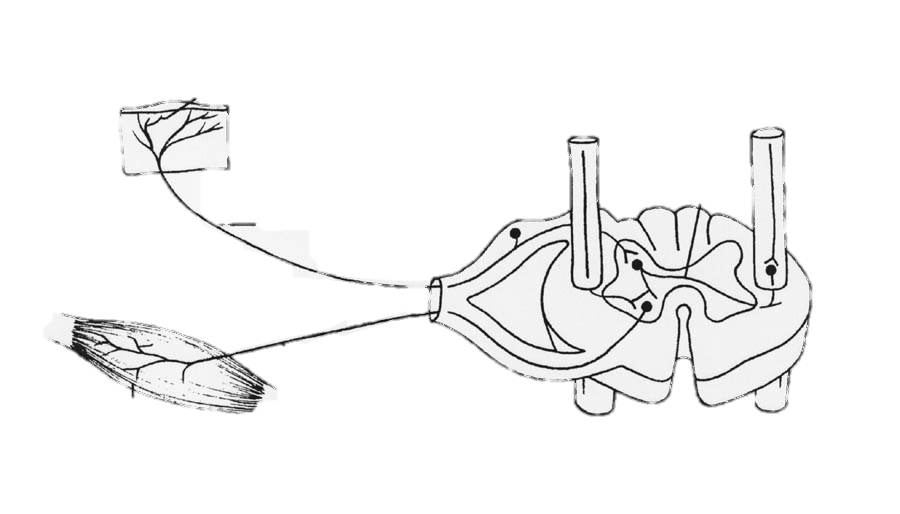
\includegraphics[width=1\columnwidth]{figs/brain2.jpg}
\caption{Analogia de sistemas reativos com o ser humano.}
\label{brain2}
\end{figure}

\section{Paradigma h�brido ou deliberativo/reativo}

Arquiteturas deliberativas e reativas apresentam vantagens e
desvantagens e que muitas vezes se op�e. Por exemplo, � muito ineficiente
utilizar uma arquitetura deliberativa em um ambiente extremamente din�mico,
assim como � ineficiente utilizar arquitetura reativa em uma linha de montagem
(manipuladores industriais). � natural pensar que integrando, de alguma forma,
as duas arquiteturas, formando uma arquitetura h�brida, ser� poss�vel absorver
as vantagens de ambas.

Atualmente, os rob�s com arquitetura h�brida predominam. Em muitas
aplica��es de rob�s m�veis mais complexas, fica claro que formas de conhecimento
do mundo na arquitetura rob�tica permitem que a navega��o dos rob�s seja mais
flex�vel, eficiente e geral. A arquitetura h�brida tenta combinar os
m�todos simb�licos da IA e seu uso de representa��o abstrata do modelo do mundo,
mas mantem o objetivo de prover robustez, resposta em tempo real e flexibilidade
dos sistemas puramente reativos. Arquiteturas h�bridas podem permitir a
reconfigura��o de controles reativos baseado no conhecimento do mundo atrav�s da
sua capacidade de raciocinar sobre os componentes comportamentais subjacentes.

O principal problema no paradigma h�brido � em como desenvolver uma
metodologia unificada de arquiteturas que garantem um sistema capaz de executar
planos de uma maneira robusta, como a arquitetura reativa, e, ao mesmo tempo,
ter um entendimento de alto n�vel da natureza do mundo e um modelo da inten��o
do usu�rio.  

\subsection{Rob�s h�bridos}

\subsection{Aquitetura h�brida}
Em \cite{arkin1998behavior}, Arkin aponta quatro estrat�gias para o
projeto de arquiteturas h�bridas:

\begin{itemize}
  \item Sele��o: o planejador � visto como um configurador. O planejador
  determina a composi��o de comportamentos e par�metros usados durante a
  execu��o. O planejador pode reconfigur�-los quando necess�rio devido a falhas
  no sistema.
  \item Conselho: o planejador � visto como um aconselhador. O planejador sugere
  mudan�as que o controle reativo pode ou n�o usar.
  \item Adapta��o: o planejador � visto como um adaptador. O planejador
  continuamente altera os componentes reativos ativos de acordo com as mudan�as
  nas condi��es do mundo e requisitos de tarefas.
  \item Adiamento: o planejador � visto como um recurso para ser usado em �ltimo
  caso. Neste caso, os planos s� s�o elaborados quando necess�rios.
\end{itemize}



\subsection{An�lise cr�tica} 

Em 1996, Healey, A. J. [8] (Autonomous Underwater Vehicle Laboratory,
California), aplica t�cnicas de controle h�brido em seu trabalho de
desenvolvimento do AUV Phoenix.  O controle h�brido ser� respons�vel tanto pela
movimenta��o do ve�culo, cont�nuo e s�ncrono, quanto pela sequ�ncia l�gica das
fases das miss�es, eventos discreto com transi��es ass�ncronas.  

Haley prop�e uma arquitetura de software h�brida com tr�s n�veis organizacionais
e hier�rquicos, figura~\ref{HEALEY_1}: 
\begin{itemize}
  \item \textbf{Estrat�gico}: utiliza Prolog como linguagem de controle de
  miss�o. Desenvolve os comandos que levam o ve�culo a executar determinada
  miss�o.
  \item \textbf{T�tico}: fun��es na linguagem C que faz interface com os
  predicados de Prolog e retorna \emph{TRUE / FALSE}. Este n�vel funciona de
  maneira ass�ncrona e ret�m os dados da miss�o, al�m de se comunicar com o
  n�vel de execu��o.
  \item \textbf{Operacional}: comanda os subsistemas do ve�culo a ativar fun��es
  de controle relacionadas ao n�vel t�tico.
\end{itemize}

\begin{figure}[h!]
\centering
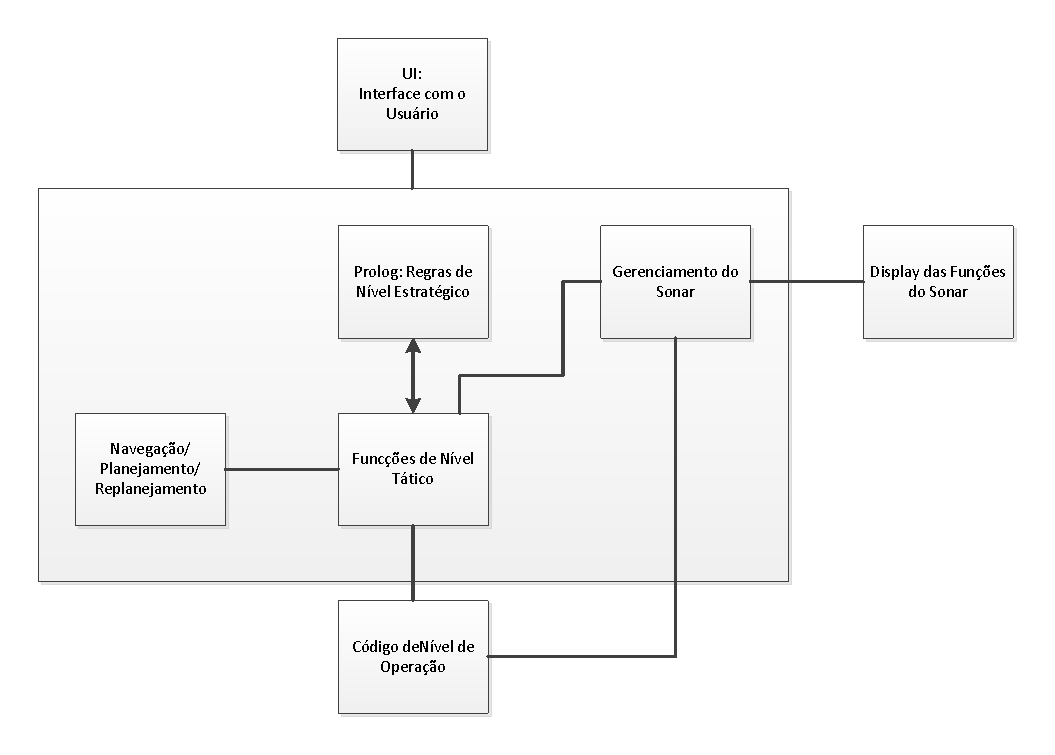
\includegraphics[width=1\columnwidth]{figs/HEALEY_1.pdf}
\caption{Arquitetura do Rob� Phoenix de Healey}
\label{HEALEY_1}
\end{figure}

Em 1996, Silva, V. et al [6] (Institute for Systems and Robotics, Lisboa),
projetaram, desenvolveram e testaram um sistema de controle de miss�o para o
MARIUS, rob� aut�nomo submarino. O trabalho de Silva, V. [6], introduz novos e
importantes conceitos chave para o MCS: Tarefa do Sistema (\emph{System Task}), Primitiva do
Ve�culo (\emph{Vechicle Primitive}), Procedimento de Miss�o (\emph{Mission Procedure})
e Programa de Miss�o (\emph{Mission Program}). Al�m disso, a arquitetura do
ve�culo, por ser um AUV, possui sistemas e interconex�es
semelhantes ao rob� DORIS, estudo desta disserta��o.

\textbf{Tarefa do Sistema} (ST): � a especifica��o param�trica de uma classe
de algoritmos ou processos que implementam uma funcionalidade b�sica em um rob�.
Requer a implementa��o de dois m�dulos: \textit{i}) um \emph{m�dulo Funcional}
que cont�m um determinado algoritmo e processo, e transfere dados com outras
Tarefas do Sistema e dispositivos f�sicos; \textit{ii}) um \emph{m�dulo
Comando}, m�quina de estado finito, que recebe comandos externos, produz
mensagens de sa�da, e controla a sele��o de algoritmos, processos, e caminhos
dos dados para/de m�dulos Funcionais.

A arquitetura do ve�culo DORIS teve grande influ�ncia da organiza��o do ve�culo
MARIUS descrita abaixo, figura~\ref{SILVA_1}:
\begin{itemize}
  \item \emph{Vehicle Support System} (VSS) - Controla a distribui��o de energia
  aos hardwares instalados no ve�culo, monitora consumo de energia e detecta
  falhas de hardware, podendo enviar comandos de emerg�ncia.
  \item \emph{Actuator Control System} (ACS) - Controla a velocidade de rota��o
  dos propulsores e posi��o dos ailerions e lemes. Os \emph{Set Points} dos
  atuadores s�o dados pelo \emph{Vehicle Guidance and Control System} (VGCS) e
  os dados dos atuadores s�o transmitidos para o \emph{Mission Control System}.
  \item \emph{Navigation System} (NS) - Estima posi��o linear e velocidade do
  ve�culo, orienta��o e velocidade angular. O sistema funde informa��es do
  \emph{Positioning System} (\emph{Long Baseline unit}) e \emph{Motion Sensor
  Integration System}, o qual inclui diversos sensores. As sa�das do NS s�o
  entradas do VGCS, e enviadas ao MCS.
  \item \emph{Vehicle Guidance and Control System} (VGCS) - Recebe como entrada
  as trajet�rias de refer�ncia pelo MCS, e os dados de navega��o do NS. Suas
  sa�das s�o \emph{Set Points} para velocidade de rota��o e outros atuadores do
  ACS, tal que o ve�culo siga a trajet�ria desejada mesmo com incertezas e
  dist�rbios.
  \item \emph{Communication System} (COMS) - Controla o link bidirecional usado
  pelo operador para passar miss�es ao MCS, e pelo ve�culo para passar status de
  miss�o ou estados do ve�culo.
  \item \emph{Environmental Inspection System} (EIS) - Coleta dados do ambiente
  com diversos sensores (inclusive c�meras), como temperatura, press�o, pH. �
  controlado pelo MCS.
  \item \emph{Data Logging System} (DLS) - Adquiri e armazena dados do ve�culo.
  \item \emph{Mission Control System} (MCS) - Sequencia e sincroniza a execu��o
  das tarefas b�sicas do ve�culo para uma determinada miss�o e prov� a
  recupera��o em caso de falhas.
\end{itemize}

\begin{figure}[h!]
\centering
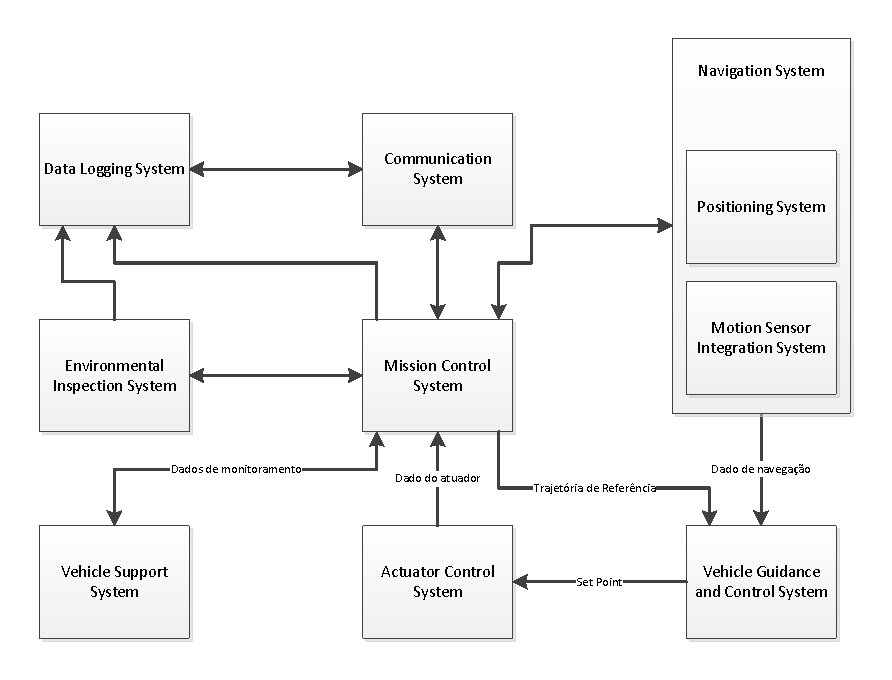
\includegraphics[width=1\columnwidth]{figs/SILVA_1.pdf}
\caption{Arquitetura do Ve�culo MARIUS}
\label{SILVA_1}
\end{figure}

Silva desenvolveu os softwares CORAL e ATOL para implementa��o das VPs e STs em
redes de Petri de forma que um usu�rio final, como um operador, pudesse
facilmente criar seus MPs. A grande contribui��o  

%TODO falar de blackboard quando for falar de ROS
Antes de Brooks, em 1983, Elfes, A. \cite{elfes1983distributed},j� havia
idealizado uma arquitetura em m�dulos e controle distribu�do a fim de atingir
efetividade em processamento paralelo, flexibilidade de intera��o com os
diversos sensores, distribuir capacidades de decis�o e flexibilidade de
expans�o e modifica��o do sistema.
Por�m o sistema de comunica��o entre m�dulos era centralizado
(\emph{Blackboard}) e s� realizavam uma determinada tarefa sob o comando de um
Plano de Controle (\emph{Control Plan}). O usu�rio ainda deveria explicitamente
codificiar paralelismo, os casos das exce��es e condi��es inesperadas.

  \chapter{Arquitetura proposta}

O cap�tulo~\ref{bibliografia} apresentou os conceitos necess�rios para o
entendimento desta disserta��o, mostrou a evolu��o das arquiteturas rob�ticas e
controles de miss�o, e as diversas aplica��es em rob�s modernos. A autonomia de
um rob� depende, em grande parte, do desenvolvimento desta arquitetura rob�tica.

Neste cap�tulo, ser� apresentada uma implementa��o da arquitetura h�brida de
tr�s camadas, utilizando o ambiente de desenvolvimento ROS, para um rob�
m�vel que executa tarefas de inspe��o, a DORIS. Como definido no
cap�tulo~\ref{bibliografia}, a arquitetura rob�tica n�o � apenas uma
arquitetura de software, mas sim uma arquitetura que depende dos
componentes f�sicos do rob� (hardware) e a sua aplica��o. Dessa forma, faz-se
necess�rio apresentar o objeto de estudo desta disserta��o.

\section{Rob� DORIS}\label{doris}
DORIS � um rob� desenvolvido pela COPPE/UFRJ, em colabora��o com Petrobras e
Statoil, para aplica��o \textit{offshore}: monitoramento e inspe��o em
plataformas de petr�leo. O rob� � controlado de maneira aut�noma ou teleoperado,
permitindo que o operador acompanhe o estado da miss�o, e monitore a informa��o
dos sensores. O rob� apresenta as seguintes funcionalidades
\cite{carvalho2013doris}:

\begin{itemize}
  \item Detec��o de anomalias por v�deo: uso de m�ltiplas c�meras (luz vis�vel,
  infravermelho, fisheye e est�reo) para detectar anomalias, como objetos abandonados, fuma�a,
  fogo, intrusos e vazamentos.
  \item Detec��o de anomalias por �udio: microfones detectam �udios an�malos,
  como explos�es, e realizam diagn�stico de mau funcionamento de m�quinas, comparando os sons recebidos com
  assinaturas obtidas previamente.
  \item Detec��o de anomalias por vibra��o: DORIS possui um manipulador com
  sensor de vibra��o em seu efetuador para inspecionar o funcionamento de m�quinas, a partir de
  algoritmos com classificadores de falhas.
  \item Detec��o de anomalias por sensor de g�s: sensor de hidrocarboneto
  detecta o vazamento de gases.
  \item Mapeamento 3D do ambiente: DORIS � capaz de reconstruir um ambiente 3D a
  partir de c�meras e Laser.
  \item Detec��o de anomalias por temperatura: DORIS possui um sensor de
  temperatura e umidade.
  \item Detec��o de anomalias por c�mera de infravermelho: uma c�mera de
  infravermelho pode detectar pessoas, indicar a presen�a de intrusos ou
  indentificar inc�ncidos.
\end{itemize}

DORIS � um rob� m�vel que se locomove em um trilho pelo uso de dois gimbals, os
quais cont�m atuadores e rodas. O rob� foi desenvolvido dentro da filosofia
de modularidade, isto �, novos sensores podem ser integrados ao sistema, ou at�
um novo m�dulo do rob� pode ser adicionado, a fim de melhorar seu desempenho
dentro do escopo da aplica��o de inspe��o. Isso exige a
flexibilidade e modularidade do sistema mec�nico, software e sistema
el�trico/eletr�nico.

O sistema � alimentado por quatro baterias, composto por um computador
embarcado com processador de alto desempenho e mem�ria, e um \textit{solid-state drive} para armazenamento. Possui
comunica��es: Wireless IEEE 802.11n com a base (operador); \textit{Controller
Area Network} (CAN) entre computador embarcado e drivers dos atuadores; rede \textit{Local
Gigabit Ethernet} para os diversos componentes internos do rob�; e r�dio 2.4/5.0
GHz para emerg�ncia. Possui atuadores: quatro motores 200 W EC-4pole para
locomo��o; e quatro motores para as juntas do mannipulador. Sensores:
c�mera fixa; c�mera t�rmica; c�mera \textit{fisheye}; duas webcams; e uma
\textit{Inertial Measurement Unit} (IMU). Al�m disso, h� um
sistema eletr�nico de suporte de ve�culo, chamado \textit{Vehicle Support
System (VSS)} \cite{freitas2015embedded}, capaz de detectar falhas eletr�nicas,
distribuir energia de maneira �tima entre os componentes e proteger o rob� em
situa��es emergenciais.

O VSS possui fun��es que independem do software e da arquitetura rob�tica, s�o
considerados de alto risco e, portanto, n�o est�o dispon�veis para
programador e usu�rio. Em detalhes, as fun��es do VSS s�o:
\begin{itemize}
  \item Detec��o de falhas: em dispositivos, pelo monitoramento de
  corrente/tens�o; no m�dulo, pela verifica��o de temperatura/umidade;
  \item Prote��o de dispositivos contra sobrecorrente gra�as a fus�veis;
  \item Distribui��o �tima de energia e monitoramento de baterias;
  \item Bot�o de emerg�ncia para desligamento manual ou via r�dio.
\end{itemize}

O trilho por onde o rob� se desloca � constru�do a partir de tubos de
policloreto de polivinila (PVC) e possui se��es retas, curvas ortogonais de
subida, descida, para a direita e para a esquerda. Os segmentos curvos s�o tubos
de 1 m dobrados $90^o$, resultando em curvaturas de aproximadamente 630 mm. Um
trilho para testes foi constru�do no Centro de Pesquisas e
Desenvolvimento da Petrobras (CENPES) e sua extens�o � cerca de 140 m.

\section{A arquitetura rob�tica implementada}

Na se��o~\ref{doris}, foi apresentado o rob� DORIS e suas funcionalidades. Como
foi definido na se��o~\ref{conceitos}, pela vis�o do autor, o conceito de
\emph{arquitetura rob�tica} n�o � equivalente apenas a uma arquitetura de
software, necessitando da avalia��o do rob� como um todo, isto �, seus
elementos de hardware e sua aplica��o. Assim como o desenvolvedor do RDE ROS
\cite{quigley2009ros} evidencia que n�o h� melhor RDE, j� que todos apresentam
vantagens e desvantagens e o melhor depende de sua aplica��o, tamb�m n�o h�
melhor arquitetura rob�tica, pois esta depende dos hardwares do rob� e tamb�m da
sua aplica��o.

DORIS � um rob� m�vel com a funcionalidade de inspe��o em um ambiente n�o muito
din�mico, usando t�cnicas que exigem grande processamento de imagem (c�meras) e
outros sensores. O usu�rio final poder�, com o aux�lio de uma interface,
programar as miss�es: inspe��o at� uma posi��o do trilho, inspe��o de
equipamento, ir at� uma posi��o do trilho, e ronda (inspe��o global). Al�m
disso, o usu�rio pode tomar o controle manual do rob�, e visualizar as
respostas dos sensores.
 
As funcionalidades de inspe��o do rob� exigem a constru��o e manuten��o do
modelo do mundo, pois h� constante compara��o com a situa��o esperada e
poss�veis anomalias. Tamb�m fica claro que n�o � s� um modelo do mundo que se
faz necess�rio, mas a constru��o de modelos distintos para cada componente
de forma a otimizar as miss�es. Al�m disso, rob�s \textit{offshore} exigem
grande robustez, por trabalharem em ambientes hostis, e que demandam a��es r�pidas em situa��es
emergenciais. As exig�ncias de um controle de miss�o para modos
flex�veis de inspe��o, a manuten��o de modelos de mundo e a robustez
no controle do rob� demandam uma arquitetura h�brida.

No cap�tulo~\ref{bibliografia}, foi explicitada algumas formas de arquitetura
h�brida, mas aquela com maior n�mero de aplica��es bem sucedidas � a arquitetura
h�brida de tr�s camadas, utilizadas desde a aplica��o do carro aut�nomo do
desafio DARPA (Stanley) at� a aplica��o de explora��o do rob� da NASA no
planeta Marte. 

Escolhida a arquitetura h�brida de tr�s camadas como arquitetura rob�tica da
DORIS, faz-se ainda necess�rio explicitar a implementa��o de cada camada, isto
�, como e qual executar� as fun��es descritas por Murphy: sequenciador,
gerenciador de recurso, cart�grafo, planejador de miss�o, e monitor de
desempenho. A arquitetura de tr�s camadas � formada por: camada Funcional,
camada Executiva e camada Planejador, e como cada arquitetura de tr�s camadas
apresenta suas peculiaridades, as camadas desenvolvidas para o rob� DORIS s�o descritas nas
subse��es adiante.


\subsection{Implementa��o da camada Funcional}

A camada funcional � a primeira implementada e exaustivamente testada no
rob� DORIS. Como nas outras arquiteturas de tr�s camadas previamente
apresentadas, a camada Funcional � o n�vel mais baixo, conecta sensores a
atuadores, implementa controladores PID, e diversos outros algoritmos, por
exemplo para a localiza��o do rob�. Utiliza-se Ubuntu/Linux como sistema
operacional e ROS como RDE para a implementa��o do n�vel funcional, j� que este
apresenta todas as vantagens descritas na subse��o~\ref{ros}, e linguagem de programa��o C++, a fim de
se garantir maior efici�ncia computacional.

A camada funcional seguiu a recomenda��o dos desenvolvedores do ROS, sendo
estruturado de maneira semelhante � camada funcional do sistema CLARAty. Neste,
a camada funcional � uma interface com todo o sistema de hardware e suas
capacidades. � um software orientado a objeto, obtendo assim modularidade de
hardware, e uma estrutura��o apropriada para usar as propriedades de
heran�a, em software. A figura~\ref{claratyfunc} mostra a organiza��o da camada
Funcional da arquitetura CLARAty.

\begin{figure}[!ht]
\centering
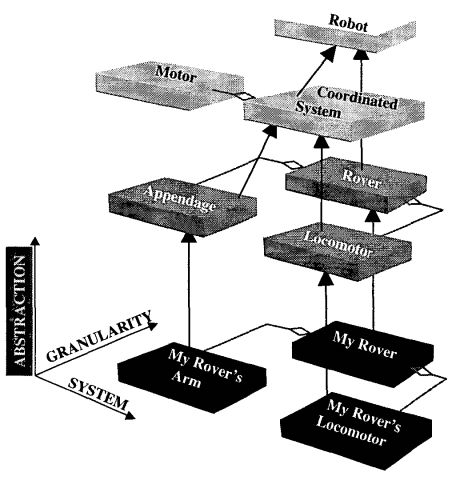
\includegraphics[width=.5\columnwidth]{figs/claratyfunc.jpg}
\caption{Organiza��o da camada Funcional CLARAty}
\label{claratyfunc}
\end{figure}

Foi proposto o \textit{Robot Package Software}. Neste sistema,
\emph{Tools} (janelas gr�ficas) e \emph{Componentes} (unidades de comunica��o e
processamento) s�o agrupados em \textit{Robot Package} (bibliotecas din�micas).
Os componentes que lidam com hardware rodam no computador embarcado do rob�,
j� os componentes que interagem com as \textit{tools} rodam no computador base.
Os diversos componentes, tanto do computador embarcado quanto da base, se
comunicam atrav�s de mensagens ROS, permitindo que a base controle o rob�, na
fun��o de teleopera��o \cite{freitas2015embedded}. Os componentes do rob� s�o
o foco de estudos desta disserta��o, j� que os componentes da base n�o est�o
diretamente ligados � autonomia do rob�, mas apenas a uma fra��o do controle de
miss�o, que diz respeito � interface com o usu�rio e \textit{feedback} dos
planos ao usu�rio.

Dois \textit{Robot Packages} fazem parte no desenvolvimento do rob� DORIS:
\textit{General Package} e \textit{DORIS Package}, derivado do primeiro. Outros
rob�s desenvolvidos por GSCAR, como o ROV LUMA, possuem seus pacotes
espec�ficos, derivados do \textit{General Package}. 

O \textit{General Package} cont�m os componentes e \textit{tools} gerais
relacionados a v�deo, �udio, tabela de dados, \textit{gamepad} (para controle
remoto de rob�s), e configura��es de dispositivos que podem ser usados em outros
rob�s

O \textit{DORIS Package} � um pacote mais espec�fico ao rob� DORIS e lida com
seus elementos de hardware e suas funcionalidades. Do ponto de vista de uma
arquitetura rob�tica, neste pacote foram implementados os \emph{comportamentos}
espec�ficos do rob� DORIS.  Os diversos componentes implementados para o DORIS
foram divididos em funcionalidades, neste trabalho, a fim de proporcionar melhor
entendimento.

Como j� descrito na se��o~\ref{doris}, os atuadores para locomo��o e para o
manipulador do DORIS se comunicam via CAN-Bus, que prov� velocidade e
transfer�ncia confi�vel dos dados \cite{corrigan2008introduction}. Esta
comunica��o extra, exigiu a implementa��o do componente \emph{CANOpen}, que utiliza a biblioteca
SocketCAN disponivel em Linux. Um componente \emph{EPOS} � classe derivada de
\emph{CANOpen} e especifica este tipo de comunica��o com o hardware EPOS
(driver) utilizado no DORIS, al�m de implementar outras caracter�siticas do
driver, como os dados dos encoders dos motores: posi��o (odometria), velocidade
e corrente.
Al�m disso, h� a \emph{EPOSNodelet}, classe derivada de \emph{EPOS}, que implementa a comunica��o ROS. A implementa��o dos
componentes respeita a sugest�o do desenvolvedor do \textit{framework}, de forma
que sempre h� a cria��o de uma classe padr�o C++ e uma classe derivada dentro do
ambiente ROS, que usa os m�todos do \textit{framework}.

Os componentes que executam o controle de locomo��o do rob� s�o:
\emph{Controller}, \emph{ControllerNodelet} (derivada de \emph{Controller}),
\emph{MotionController} (derivada de \emph{Controller}),
\emph{MotionControllerNodelet} (derivada de \emph{MotionController}),
\emph{PositionController} (derivada de \emph{Controller}) e
\emph{PositionControllerNodelet} (derivada de \emph{PositionController}). Os
componentes \emph{Controller} e \emph{ControllerNodelet} (componente
\emph{Controller} com os recursos de ROS) s�o classes gen�ricas de controle,
sendo necess�ria a implementa��o do controle para o rob� espec�fico,
componentes \emph{MotionController} e \emph{PositionController}.

Os quatro hardwares EPOS possuem uma malha de controle PD ou
PID para realizar o controle do rob� por velocidade ou corrente, por�m de
maneira independente para cada motor. A sincronia e ajustes dessas malhas de
controle s�o realizados no componente \emph{MotionController}. Este componente
se comunica por servi�o de ROS (\textit{service}) com o componente
\emph{EPOSNodelet}, enviando os valores de velocidade desejados para cada motor.
Por exemplo, observe que, em uma curva, devido � dist�ncia entre os dois gimbals
do rob� e � dist�ncia entre as rodas dos gimbals, os motores devem possuir
velocidades diferentes. O \emph{MotionController} envia set-points de
velocidade �s EPOS e pode alterar os par�metros de acelera��o e
desacelera��o. Al�m disso, este componente � respons�vel por receber entradas do
componente \emph{Joystick} e \emph{Interface}, que podem controlar o rob� pela
base, ou \emph{MissionController}, o componente de miss�o aut�noma. H� apenas
a prioridade do \emph{MissionController} sobre todos os outros controladores,
tal que, com exce��o do \emph{MissionController}, o componente que ir�
controlar ser� o primeiro que pedir o controle.

O componente \emph{PositionController} ser� futuramente integrado ao
\emph{MotionController}. Sua funcionalidade � realizar um controle de posi��o,
logo possui uma malha interna de controle, n�o dispon�vel no hardware da EPOS, e
se comunica com o componente \emph{MotionController}, enviando set-points de
velocidades. � um controle proporcional de posi��o com satura��o de velocidade.

O manipulador da DORIS utiliza mais quatro EPOS (quatro motores) e exigir� ainda
a implementa��o de um controle de for�a para sensoriamento de equipamentos ao
toque, a partir de um sensor de vibra��o. Componentes como \emph{ForceControl} e
\emph{InspectionVibration} ainda est�o em desenvolvimento em.
%TODO referencia marco

Ainda em fase de aperfei�oamento, os componentes de localiza��o
\emph{Localization} e \emph{LocalizationNodelet} recebem mensagens de ROS
(\textit{subscriber}) do componente \emph{EPOSNodelet}, os dados da odometria,
isto �, quanto cada roda girou. Dentro de \emph{Localization} � feita uma m�dia
para estimar quanto o rob� se locomoveu. Em implementa��o, est� sendo feito um
sistema inteligente de localiza��o com os dados dos sensores IMU e LaserScan. A
fus�o de sensores permitir� estimar de maneira precisa a posi��o do rob�. O
\emph{LocalizationNodelet} ainda envia mensagens (\emph{Publish}) para o
\emph{PositionController}, \emph{MotionController} e \emph{RVIZ}, um componente
de vizualiza��o para o usu�rio.

Os diversos componentes de sensores, no rob�, s�o: \emph{AudioSender},
\emph{AudioSenderNodelet} (derivada de \emph{AudioSender}),
\emph{VideoSender}, \emph{VideoSenderNodelet} (derivada de
\emph{VideoSender}), \emph{VideoWebcamera} (derivada de
\emph{VideoSenderNodelet}), \emph{AxisVideo} (derivada de
\emph{VideoSenderNodelet}), \emph{LMS1xx}, \emph{IMU}, \emph{IMUNodelet} e
\emph{ColorDetector}.

O componente \emph{AudioSender} � um driver que faz a interface com os diversos
microfone dispon�veis no rob�. Comunica-se (\textit{publisher}) por mensagem de
ROS com o componente da base \emph{AudioReceiverNodelet} (\textit{subscriber})
para disponibilizar os dados ao usu�rio. Futuramente, ir� se comunicar
(\textit{publisher}) com o \emph{InspectionAudioNodelet} (\textit{subscriber}),
um componente que compara o �udio da base de dados do rob� e detecta anomalias atrav�s de um algoritmo de reconhecimento de padr�es.

O componente \emph{VideoWebcamera} � um driver que faz a interface com as duas
c�meras webcams dispon�veis no rob�. Comunica-se
(\textit{publisher}) com o componente da base
\emph{VideoReceiverNodelet} (\textit{subscriber}) para disponibilizar os dados
ao usu�rio, e com o componente \emph{ColorDetection} (\textit{subscriber}), um
algoritmo que verifica a porcentagem de vermelho obtida em cada frame da
c�mera. Futuramente, o componente \emph{ColorDetection} ir� se comunicar
(\textit{publisher}) com o \emph{Localization} (\textit{subscriber}), j� que a
informa��o de vermelho no trilho ser� utilizada para calibrar a
localiza��o.

O componente \emph{LMS1xx} � um driver que faz a interface com o LaserScan,
sensor que realiza um escaneamento a laser do ambiente. Comunica-se
(\textit{publisher}) com o componente da base \emph{LaserReceiverNodelet}
(\textit{subscriber}) para disponibilizar os dados ao usu�rio. Futuramente, ir�
tamb�m se comunicar com o \emph{PoleDetection} (\textit{subscriber}), que possui
um algoritmo para detec��o de postes, e o \emph{Localization} (\textit{subscriber}), j� que
este � mais um sensor que prov� dados para o sistema de localiza��o (altura do
rob�).

O componente \emph{IMU} � um driver que faz a interface com a IMU.
Ele envia uma lista de dados: velocidade, orienta��o, posi��o, p�los
magn�ticos e outros. Futuramente, tamb�m ir� se comunicar com o
\emph{Localization}.

O componente \emph{AxisVideo} � um driver que faz a interface com a c�mera fixa
da AXIS. Comunica-se (\textit{publisher}) com o componente
da base de mesmo nome para disponibilizar os dados ao usu�rio. Futuramente, o
algoritmo de detec��o de anomalias por v�deo ser� integrado ao sistema ROS,
logo um componente \emph{InspectionVideo} ser� \emph{subscriber} do mesmo
t�pico.

A FIGURA represente o esquema de comunica��o entre os diversos componentes e
suas hierarquias.

\subsection{Implementa��o da camada Executivo}
%TODO falar das prioridades
%TODO recursos compartilhados, como fica?
%TODO Referenciar DFKI tb
A camada Executivo elaborada para a DORIS usa SMACH (subse��o~\ref{smach}) como
linguagem da camada Executivo, e implementa a t�cnica de fun��o de coordena��o
competitiva (subse��o~\ref{reativa}), a arquitetura de subsun��o, onde o m�dulo
b�sico de comportamento reativo � uma m�quina de estados aumentada
(\emph{AFSM}) da figura~\ref{afsm} sem \textit{Reset}. A camada Executivo � o
foco da implementa��o do autor desta disserta��o e, junto com a camada
Planejador, permite a autonomia do rob�.

As subse��es a seguir detalham a implementa��o da camada Executivo,
identificando como � realizada cada responsabilidade: Tradutor (planos do
Planejador em tarefas), Sequenciador, Selecionador, Gerenciador de recursos, e
Monitoramento da execu��o e recupera��o de erros (\textit{Execution monitoring
and error recovery}). Como o ambiente de desenvolvimento da camada Funcional �
ROS, optou-se pela utiliza��o da camada Executivo SMACH \cite{bohren2010smach}
por demonstrar resultados positivos em diversas aplica��es, e j� ser integrada
ao sistema ROS. Foram adicionadas algumas funcionalidades � camada a fim de
garantir todas as responsabilidades de uma camada Executivo. A linguagem de
programa��o utilizada � Python.


\subsubsection{Sequenciador e Selecionador}
SMACH � um \textit{framework} para projetar m�quinas de estados hier�rquicas
concorrentes. As m�quinas de estados de SMACH possuem caracter�sticas bem
peculiares n�o encontradas em m�quinas de estados formais, como a \textit{user
data}, comentada na subse��o~\ref{smach}. O Sequenciador desenvolvido para a
DORIS utilizar� as capacidades de SMACH para a modelagem das tarefas do rob�.

Dependendo da aplica��o, rob�s, como seres humanos, possuem um conjunto de
processos que est�o sempre em execu��o, e outros conjuntos de processos que s�
entrar�o em execu��o dependendo da tarefa que o rob� ir� executar. Por exemplo,
em um ser humano, os processos vitais como ``respirar'' e ``o bombear do
cora��o'' est�o sempre em execu��o, sendo que alguns podem ser postos em espera
por um tempo, como ``respirar'', e outros s�o incontrol�veis, como ``o bombear
do cora��o''. A camada Executivo � a camada, em DORIS, que assumir�
esta responsabilidade de \textbf{Selecionador}, simulando este mesmo princ�pio
encontrado na natureza, extremamente necess�rio para garantir robustez e
prote��o. 

 


A concep��o da camada Executivo � de se criar v�rios processos sendo executados
em


\subsubsection{Gerenciador de recursos}


\subsubsection{Monitoramento de tarefas e recupera��o de
erros}\label{monitoamento}
% The languages presented differ considerably in how
% they deal with execution monitoring and exception
% handling. ESL and TDL both provide explicit
% execution monitoring constructs and support exceptions
% that are thrown and then caught by registered
% handlers in a hierarchical fashion. This type of
% exception handling is similar to that used in C++, Java,
% and Lisp. ESL and TDL also support clean up
% procedures that can be invoked when tasks are
% terminated. RAPs and PLEXIL use return values to
% signal failure, and do not have hierarchical exception
% handling. PLEXIL, though, does support clean up
% procedures that are run when tasks fail. PRS has
% support for execution monitoring, but not exception
% handling. ESL and PRS support the notion of resources
% that can be shared. Both provide support for
% automatically preventing contention amongst tasks for
% the resources. In the other executive languages, this
% must be implemented separately (although there are
% plans to extend PLEXIL in this area).





\subsection{Implementa��o da camada Planejador}\label{planejador}
%TODO lembrar de mapa de equipamentos e quais precisam de manipulador
%TODO mapa de postes
%TODO mapa de distancias ao chao
%TODO mapa 3D
%TODO mapas analiticos
%TODO mapa das se��es do trilho.
%TODO mapa audio
%TODO Mapa audio de anomalias
%TODO Mapa de equipamentos
%TODO falar de SLAM

% Many architectures provide for specialized planning
% ``experts" that are capable of solving particular
% problems efficiently.
% In particular, these include
% motion planners, such as path planners and trajectory
% planners.
% Sometimes, the planning layer of the
% architecture invokes these specialized planners directly;
% in other architectural styles, the motion planners are
% part of the lower levels of the architecture (the
% executive, or even the behavioral layer). Where to put
% these specialized planners is often a question of style
% and performance (see Section 8.5).
\subsubsection{Controle de miss�o} %UI

\subsubsection{Planejador de miss�o e Tradutor}
A camada Planejador enviar� miss�es � camada Executivo, quando estas estiverem
agendadas ou quando o usu�rio requisitar. Na subse��o~\ref{hibrida}, em
\ref{murphy}, foi exemplificada a responsabilidade de \textbf{Tradutor} da
camada Planejador com um rob� assistente que serve caf�s. A implementa��o desta
responsabilidade no DORIS � realizada por um dicion�rio codificado no rob�.
Este m�todo � normalmente conhecido na literatura como \textit{encoded
knowledge} (conhecimento codificado), que s�o dados incorporados ao c�digo
fonte \textit{hard coded}.

As miss�es do rob� podem ser classificadas em: \textbf{Miss�es Simples},
\textbf{Miss�es Complexas} e \textbf{Miss�es Desconhecidas}. Todas as miss�es
possuem \textit{argumentos}, entradas m�nimas do usu�rio necess�rios para a
execu��o da miss�o.

As miss�es simples n�o necessitam de tradu��o por j� estarem em n�vel
m�nimo de m�quinas de estados SMACH. Por exemplo:
\begin{itemize}
  \item \textbf{GOTO}: miss�o de locomo��o do rob� at� um ponto do trilho. Os
  \textit{argumentos} para esta miss�o s�o: posi��o desejada no trilho, em valor
  absoluto; velocidade desejada, um valor fuzzy: ``slow'' (devagar), ``normal''
  (normal) ou ``fast'' (r�pida); dire��o de movimento, 1 para sentido de
  locomo��o para frente (baterias chegam por �ltimo) e -1 para sentido
  contr�rio; n�mero de voltas desejado, em caso de trilho fechado, antes de o
  rob� atingir a posi��o requisitada. O �nico argumento obrigat�rio � posi��o
  desejada, de forma que os valores padr�o s�o: velocidade ``fast''; dire��o de
  movimento de velocidade m�nima; e zero voltas.
  \item \textbf{RECORD\_TYPE}: gravar dados de sensores no rob�. H� um 
 \textit{argumentos} para esta miss�o que pode ser preenchido como: v�deo, �udio
 e termografia. Cada tipo representa uma miss�o de gravar dados de um sensor
 espec�fico (c�mera, microfone e c�mera termogr�fica, respectivamente).
  \item \textbf{STOP\_RECORD\_TYPE}: parar grava��o de dados de sensores no
  rob�. Assim como a inicializa��o da miss�o, h� um \textit{argumento} que deve
  ser preenchido: o tipo de grava��o, que ir� resultar na utiliza��o do sensor
  apropriado para a execu��o da tarefa.
  \item \textbf{START\_DETECTING\_ANOMALIES\_TYPE}: iniciar algum detector
  espec�fico de anomalia. H� tr�s tipos de detec��o de anomalias
  que podem ser escolhidos: v�deo, �udio e termografia. Para cada um deles, h�
  uma m�quina de estados espec�fica: iniciar algoritmo detector de anomalias por
  c�mera, microfones ou c�mera termogr�fica, respectivamente.
  \item \textbf{END\_DETECTING\_ANOMALIES\_TYPE}: finalizar algum detector
  espec�fico de anomalia. Assim como iniciar, finalizar apresenta os mesmos tr�s
  tipos de detec��o de anomalias: v�deo, �udio e termografia. E Para cada um
  deles, h� uma m�quina de estados espec�fica: iniciar algoritmo detector de
  anomalias por c�mera, microfones ou c�mera termogr�fica, respectivamente.
\end{itemize}

As miss�es complexas, de mais alto n�vel, s�o combina��es de
miss�es simples. Estas necessitam ser traduzidas pelo Planejador com os
argumentos corretos. Por exemplo:
\begin{itemize}
  \item \textbf{GOTO\_BASE}: miss�o de locomo��o do rob� � base.
  N�o h� \textit{argumentos} para esta miss�o. Tradu��o necess�ria para camada
  Executivo: \textbf{GOTO}: posi��o zero, velocidade ``fast''.
  \item \textbf{INSPECTION}: miss�o para inspecionar planta em um trecho.
  Necessita que o usu�rio escolha at� onde inspecionar (posi��o final absoluta
  no trilho) e o tipo de inspe��o: v�deo, �udio e termogr�fico. Tradu��o: para cada tipo selecionado realizar
  \textbf{START\_DETECTING\_ANOMALIES\_TYPE}; \textbf{GOTO}:
  velocidade ``slow'' (observe que inspe��o requer velocidade m�nima); para cada
  tipo realizar \textbf{STOP\_DETECTING\_ANOMALIES\_TYPE}.
  \item \textbf{PATROL}: realizar uma ronda completa, isto �, inspecionar toda a
  planta. N�o h� \textit{argumentos} para esta miss�o. Tradu��o:
  \textbf{INSPECTION}: todos os sensores, posi��o final do trilho.
  \item \textbf{MANIPULATOR\_INSPECTION}: inspecionar um equipamento com
  manipulador. O \textit{argumento} desta miss�o � o equipamento a
  ser inspecionado. O rob� deve ir � posi��o que se encontra o equipamento, tocar o
  equipamento com o sensor de vibra��o atrav�s do manipulador, e executar uma
  detec��o de anomalias por vibra��o. Em linguagem da camada Executivo, seria
  \textbf{GOTO}: posi��o do equipamento (requer verificar mapa de equipamentos),
  velocidade ``fast''; \textbf{MANIPULATOR\_POSITION\_CONTROL}: posi��o
  referente ao equipamento; \textbf{MANIPULATOR\_FORCE\_CONTROL};
  \textbf{START\_DETECTING\_ANOMALIES\_VIBRATION}.
\end{itemize}  

As miss�es desconhecidas s�o miss�es que n�o est�o
descritas no rob�, isto �, miss�es que, at� o momento, n�o pertencem ao
dicion�rio do rob�. At� esta fase da implementa��o, DORIS n�o permite que o
usu�rio use miss�es desconhecidas. O motivo principal disso � que o rob� n�o
interage com o ser humano de maneira direta, mas apenas atrav�s de uma
interface. Vale, por�m, explicitar situa��es de aplica��es rob�ticas em que
miss�es desconhecidas s�o essenciais:

\begin{enumerate}
  \item Rob� que serve bebidas: uma miss�o desconhecida � o usu�rio pedir
  uma bebida que n�o exista em sua base de conhecimento (mapa de bebidas).
  Durante a tarefa de reconhecer a bebida na geladeira, o rob� ir� falhar. Por�m, o Planejador
  poderia executar uma busca por fotos de bebida em algum site de buscas, antes
  de executar a tarefa, e atualizar a sua base de conhecimento (mapa de
  bebidas), de forma que a tarefa tenha resultado positivo com novo dado.
  \item J.A.R.V.I.S., a intelig�ncia artificial das hist�rias em quadrinhos
  Iron Man (homem de ferro): comandos por voz normalmente s�o complexos, j� que
  h� diversas maneiras de pedir que um plano a um rob�. Pro exemplo, os planos
  ``Rob�, preciso de uma tesoura'', ``Rob�, d�-me uma tesoura'', ``Rob�,
  traga-me uma tesoura'' s�o planos equivalentes, ditos de maneira diferentes.
  Todas estas diferentes formas devem estar dispon�veis em alguma base de
  conhecimento, dentro ou fora do rob�, como na nuvem (\textit{cloud}), a qual
  deveria ser compartilhada com todos os rob�s que exercem a mesma fun��o.
  RoboEarth \cite{hunziker2013rapyuta} � uma ideia vision�ria que est� buscando
  criar uma \textit{internet dos rob�s} (como a \textit{internet das coisas}),
  j� est� sendo integrada ao ambiente ROS, e sua contribui��o � criar um
  reposit�rio na nuvem com miss�es compartilhadas para todos os rob�s que a
  utilizam.
\end{enumerate}

\subsubsection{Agendador}

\subsubsection{Cart�grafo}
  \chapter{Resultados e Discuss�es}\label{result}

O cap�tulo~\ref{arquipro} detalhou a implementa��o das camadas da
arquitetura rob�tica h�brida de tr�s camadas. O detalhamento da implementa��o
mostrou o car�ter modular da arquitetura, o que torna poss�vel o
desenvolvimento da solu��o em est�gios independentes de programa��o. A
integra��o das camadas � trivial pelo \textit{framework} ROS e seu estilo
simples de comunica��o entre os componenetes de software.

A modularidade da arquitetura permite a avalia��o independente de cada camada e,
por fim, a integra��o � apenas um teste de comunica��o entre as camadas. Os
testes da camada Funcional, no entanto, requerem o hardware, isto �, o rob�
DORIS. Os testes da camada Executivo e Planejador podem ser simuladas em
ambiente de programa��o. Na se��o~\ref{avametodologia} deste cap�tulo, ser�
desenvolvida uma metodologia para a avalia��o da arquitetura h�brida de tr�s
camadas e as se��es seguintes, \ref{avafuncional}, \ref{avaexecutivo},
\ref{avaplanejador}, resumem os testes de cada camada.

\section{Metodologia para avalia��o das camadas}\label{avametodologia}

H� diversos crit�rios de avalia��o de uma arquitetura rob�tica. De acordo com
Arkin \cite{arkin1998behavior}, podemos avaliar arquiteturas quanto a:
\begin{itemize}
  \item \textbf{Suporte a paralelismo}.
  \item \textbf{\textit{Hardware targetability}}: este conceito se refere a
  qu�o bem uma arquitetura pode ser mapeada em sistemas rob�ticos reais, isto �,
  sensores e atuadores f�sicos; e o desempenho computacional. Este crit�rio �
  exclusivo da camada Funcional.
  \item \textbf{\textit{Niche targetability}}: qu�o bem uma arquitetura � capaz
  de fazer o rob� se adaptar ao seu ambiente de opera��o.
  \item \textbf{Suporte a modularidade}: desde a facilidade de encapsulamento de
  comportamentos abstratos e componentes (baixo n�vel) � possibilidade de
  reutiliza��o da arquitetura para outros rob�s (alto n�vel).
  \item \textbf{Robustez}: em caso de falha de hardwares (sensores, atuadores e
  etc), a arquitetura deve ser capaz de se recuperar. Quais os mecanismos que a
  arquitetura possui para contornar falhas?
  \item \textbf{Tempo de desenvolvimento}: quais as ferramentas e
  \textit{frameworks} dispon�veis na arquitetura. 
  \item \textbf{Flexibilidade em tempo de execu��o}: como o sistema de controle
  pode ser ajustado ou reconfigurado em tempo de execu��o.
  \item \textbf{Desempenho em executar tarefas}.
\end{itemize}

A arquitetura h�brida de tr�s camadas foi idealizada para passar com �tima
avalia��o em todos os crit�rios de Arkin. Entretanto, como j� explicitado na
subse��o~\ref{3t}, h� diversas formas de implementar esta arquitetura e esta
liberdade de programa��o acaba por n�o garantir boa avalia��o nos crit�rios
estabelecidos. � importante que as camadas sejam projetadas a cumprirem os
crit�rios de forma satisfat�ria.

As camadas desenvolvidas para a DORIS foram projetadas para passar
satisfatoriamente nos crit�rios de Arkin e de outros roboticistas. Dessa forma,
a metodologia de avalia��o e testes � verificar o desempenho nos crit�rios e
destacar as responsabilidades implementadas em cada camada e como elas cumprem os requisitos.

As camadas Executivo e Planejador comp�em o sistema aut�nomo do rob�. Por
mais robusto que o sistema seja, e mesmo que haja possibilidade de suspender
a��es em tempo real, as camadas de n�vel superior devem ser exaustivamente
simuladas em ambientes de programa��o e em computador semelhante ao embarcado
no rob�. Como a camada Funcional � a camada que faz interface com os hardwares
do rob� (sensores e atuadores), simula��es n�o bastam para a avalia��o dos
crit�rios de Arkin, logo s�o necess�rios testes exaustivos, em campo, com o
rob�.

\section{Testes da implementa��o da camada Funcional}\label{avafuncional}

A camada funcional � a primeira a ser implementada na camada da arquitetura
h�brida de tr�s camadas. Somente com a camada funcional � poss�vel
enviar comandos aos atuadores, ou seja, controlar o rob� por \textit{joystick}
ou com uma interface simples de usu�rio. � poss�vel observar os dados dos
sensores, processar os dados e testar funcionalidades b�sicas do rob�. 

A camada Funcional desenvolvida para DORIS � detalhada na
subse��o~\ref{camadafuncional} e, como j� foi analisada, segue o modelo
``ideal'' de implementa��o de uma camada Funcional descrita por Quigley
\cite{quigley2009ros}, desenvolvedor do ROS, e Volpe \cite{volpe2001claraty},
desenvolvedor do CLARAty. H� pacotes gen�ricos a serem atribuidos a qualquer
rob�, pacotes espec�ficos da DORIS e pacotes com funcionalidades ROS.

Com o aux�lio das \textit{tools} (subse��o~\ref{camadafuncional}), componentes
gr�ficos para o operador enviar comandos ao rob�, o usu�rio pode teleoperar o
rob� e observar as sa�das dos sensores. A figura~\ref{teleop} mostra a
teleopera��o do SAM (\textit{Single Autonomous System}), predecessor da DORIS,
em uma interface web. Na figura, pode-se observar a imagem enviada pela c�mera
interna do rob� e o ambiente 3D em que o rob� est� inserido, em RVIZ. Na
figura~\ref{robotgui}, mostram-se a interface de controle da DORIS com dados de
corrente e velocidade dos motores, a sa�da de v�deo da c�mera interna ao rob�,
e a sa�da de v�deo de uma c�mera externa ao rob�.

A camada Funcional desenvolvida no \textit{framework} ROS mostrou
\textbf{\textit{Hardware targetability}}. Al�m de ROS possuir um grande
reposit�rio de drivers (interface hardware-software), os componentes espec�ficos
desenvolvidos apresentaram �timo desempenho. 

O \textit{framework} ROS � uma ferramenta que, usada de maneira correta, faz com
que a camada Funcional passe por quase todos os crit�rios de Arkin. Podemos
avaliar a camada Funcional com os crit�rios estabelecidos:
\begin{itemize}
  \item \textbf{Suporte a paralelismo}: � inerente a sistemas
  \textit{multi-thread} (computadores embarcados com sistemas operacionais que
  permitem o paralelismo), e aos estilos de comunica��o \textit{publish-subscriber} e \textit{service}, que
  permitem que os componentes obtenham, ao mesmo tempo, acesso aos diversos dados de sensores do rob�.
\item \textbf{\textit{Hardware targetability}}: os diversos rob�s que utilizam
ROS j� mostram por si s� o \textbf{\textit{Hardware targetability}} desta
ferramenta.
\item \textbf{\textit{Niche targetability}}: ROS tamb�m j� foi utilizado por uma
variedade de aplica��es rob�ticas. Al�m disso, os resultados em DORIS mostram
que o c�digo implementado pode ser estendido a rob�s com desafios semelhantes.
\item \textbf{Suporte � modularidade}: os componentes e pacotes desenvolvidos
s�o modulares e seu n�vel de abstra��o permite a utiliza��o em outros rob�s. O
esquema de classes e heran�a � essencial para alcan�ar este objetivo.
\item \textbf{Robustez}: em caso de falha, a camada n�o entra em colapso e
mensagens de falha s�o enviadas a camadas superiores (Executivo e Planejador).
Mas a camada Funcional n�o � projetada para recupera��o de falhas,
responsabilidade de camadas superiores.
\item \textbf{Tempo de desenvolvimento}: o grande reposit�rio dispon�vel para o
\textit{framework} ROS reduz muito o tempo de desenvolvimento. Al�m disso, uma
metodologia de programa��o, e a separa��o em m�dulos facilita o desenvolvimento
de sistemas rob�ticos.
\item \textbf{Flexibilidade em tempo de execu��o}: os resultados de DORIS com a
teleopera��o mostrou que pode ser controlada com altera��o dos par�metros
de controle em tempo real. O sistema de comunica��o de ROS permite a
implementa��o de \textit{tools} que se comunicam com os componentes do rob� (
intera��o base-rob�) e cria esta flexiblidade em tempo de execu��o.
\item \textbf{Desempenho em executar tarefas}: os resultados bem
sucedidos mostraram o alto desempenho da DORIS. 
\end{itemize}
 

\begin{figure}[!ht]
\centering
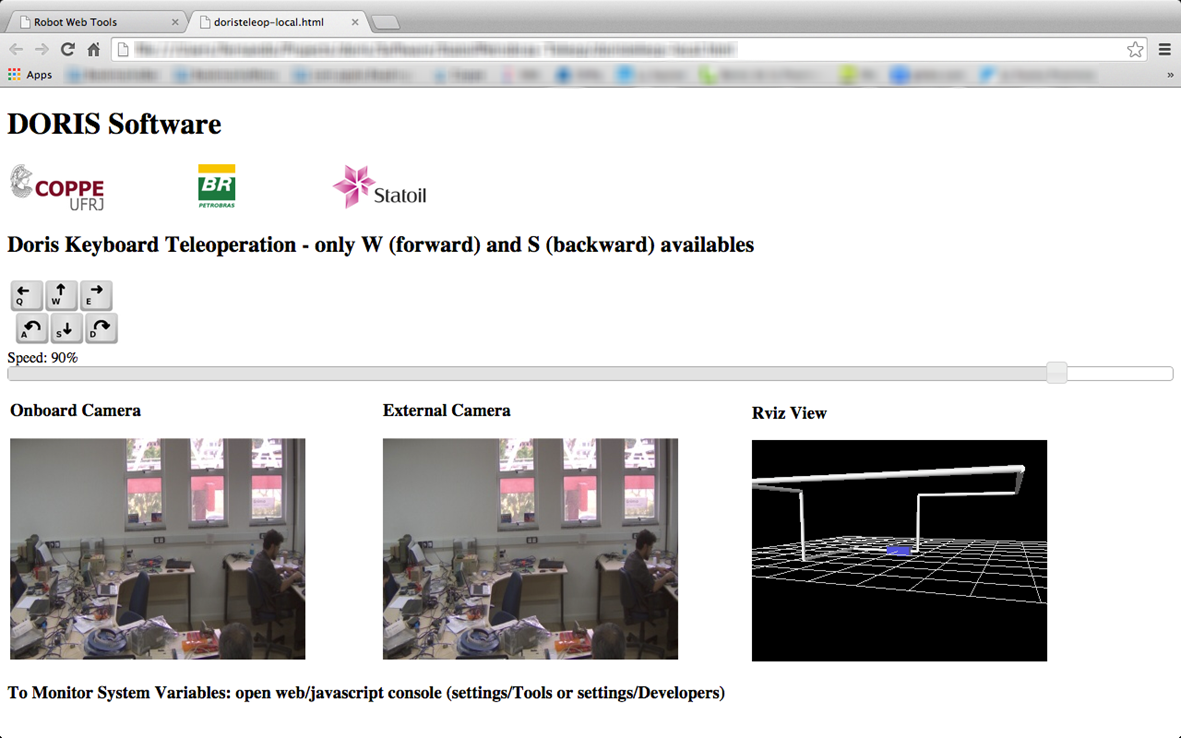
\includegraphics[width=1\columnwidth]{figs/DORIS/teleop.png}
\caption{Teleopera��o da DORIS.}
\label{teleop}
\end{figure}  

\begin{figure}[!ht]
\centering
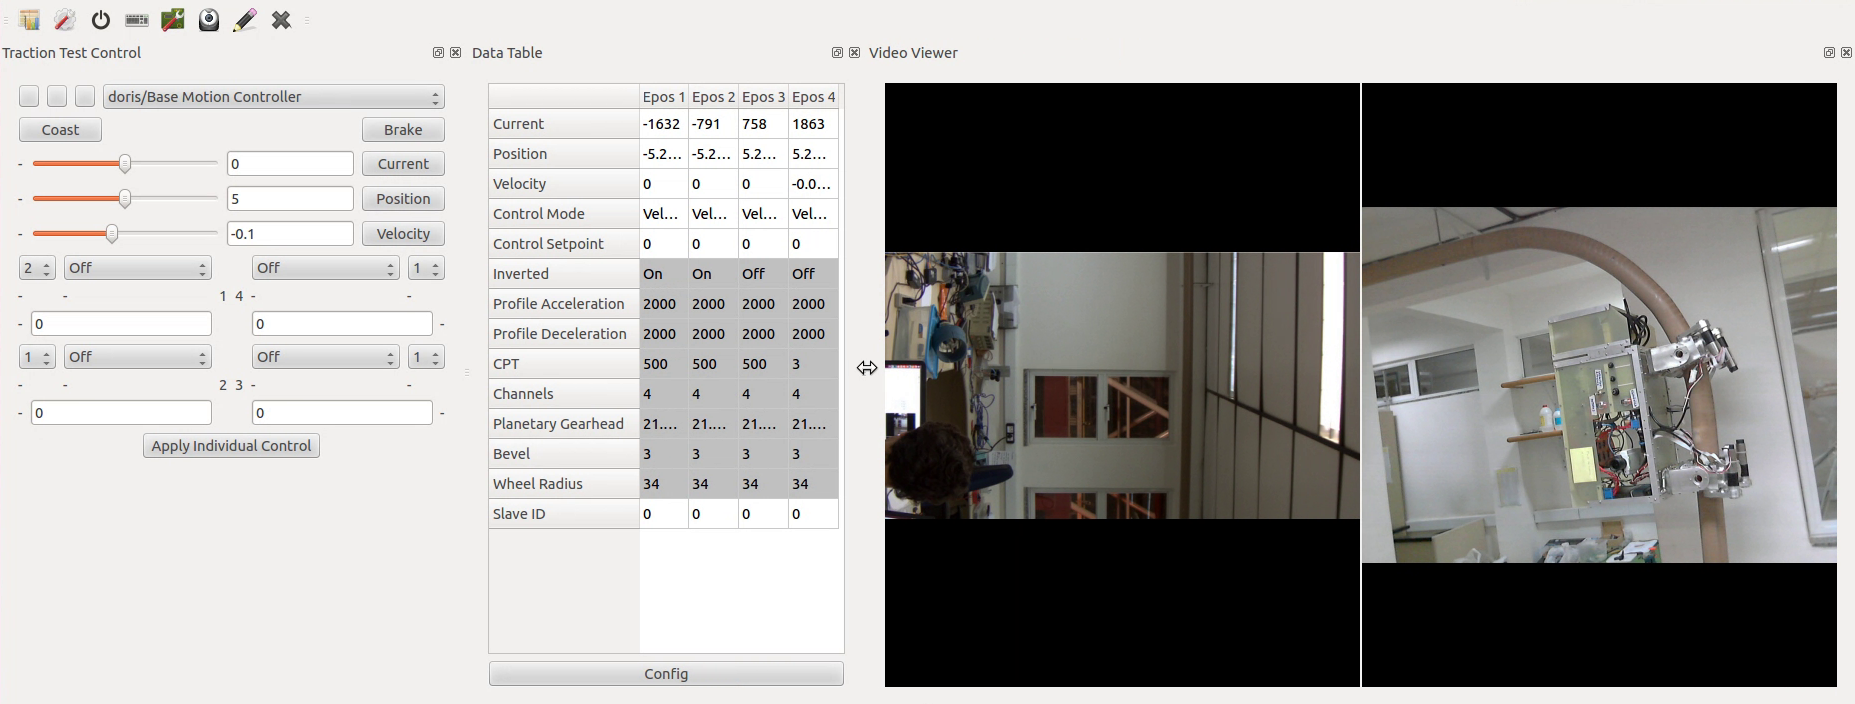
\includegraphics[width=1\columnwidth]{figs/DORIS/robotgui2.png}
\caption{Interface de controle da DORIS.}
\label{robotgui}
\end{figure}

A camada Funcional permite, por si s�, a teleopera��o do rob� e testes com o
sistema. Apesar de passar com excel�ncia pelos crit�rios
de Arkin, a camada n�o transforma DORIS em um sistema aut�nomo. As outras
camadas, al�m de garantirem esta nova configura��o do sistema, devem tamb�m
cumprir os crit�rios de Arkin. 

%TODO Futuro algoritmos do cartografo na camada funcional

\subsection{Testes de planejamento de velocidades}

Apesar de pertencer � camada Funcional da arquitetura proposta, o planejamento
de velocidades � um \textit{thread} que pertence ao desenvolvimento de um
sistema aut�nomo. O planejamento de velocidades � um algoritmo cuja sa�da
s�o as velocidades para cada trecho do trilho, ele n�o se comunica com outros
elementos da camada Funcional, n�o � interface ou driver, mas comunica-se com
componentes das camadas Executivo e Planejador. Dessa forma, como as camadas de
n�vel superior, o algoritmo � simulado, em vez de ser testado exaustivamente no
rob�.

Como j� documentado na subse��o~\ref{masterplanning}, a fun��o
\textbf{MasterPlanning} possui os argumentos: localiza��o
atual do rob�; localiza��o objetivo; dire��o de movimento (1 ou -1 - sentido
natural ou sentido contr�rio); n�mero de voltas desejado antes de chegar �
localiza��o objetivo; e se o trilho � circular (verdadeiro ou falso). A sa�da do
algoritmo � uma matriz com $n$ linhas e tr�s colunas: a primeira coluna
representa a posi��o do trilho onde ocorre troca de velocidade m�xima; a segunda coluna � a
velocidade m�xima; a terceira � o \textit{set-point} de posi��o.

\textbf{Exemplo}

Suponha que o rob� est� na posi��o 0 do trilho e come�a a execu��o da tarefa
\textit{Motion\_Planning\_Position} da miss�o \textit{GOTO(10,'fast')} (ver
subse��o~\ref{missioncontrol}).
A fun��o $master\_planning(0,'fast',10)$ retorna a matriz~\ref{matrizvmax}, que pode ser
interpretada graficamente em ~\ref{plvl}. 

\begin{table}[!ht]
\centering
\caption{Matriz de velocidades m�ximas em cada trecho do trilho do ponto 0 ao
10.}
\label{matrizvmax}
\begin{tabular}{ccc}
\hline
\multicolumn{1}{l}{Ponto de troca (m)} & \multicolumn{1}{l}{$V_{max}$ (m/s)} &
\multicolumn{1}{l}{Set-point (m)} \\ \hline 0                                  &
0.6                           & 10                            \\
1.907                              & 0.42                          & 10                            \\
3.355                              & 0.3                           & 10                            \\
4.495                              & 0.42                          & 10                            \\
5.506                              & 0.6                           & 10                            \\
5.847                              & 0.51                          & 10                            \\
7.308                              & 0.6                           & 10                            \\
8.334                              & 0.42                          & 10                            \\
9.282                              & 0.3                           & 10                           
\end{tabular}
\end{table}

\begin{figure}[!ht]
\centering
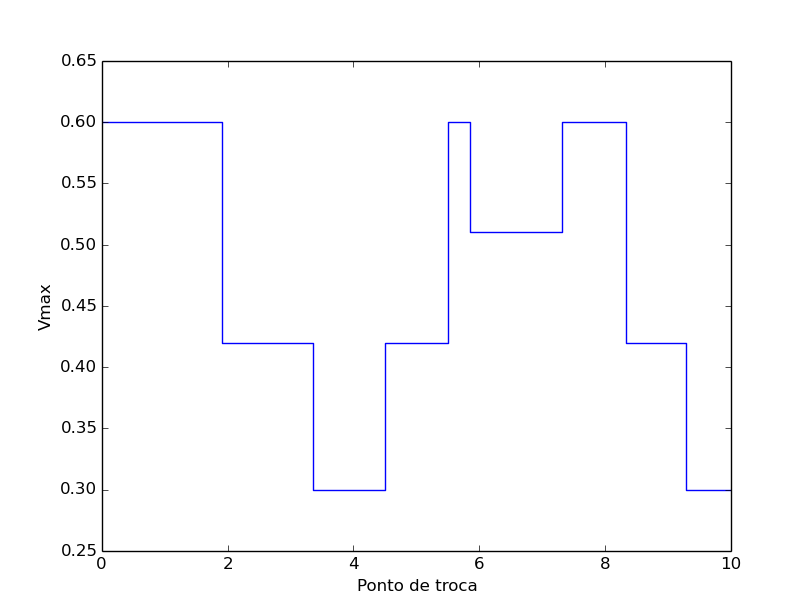
\includegraphics[width=.8\columnwidth]{figs/masterplot.png}
\caption{representa��o gr�fica do plano de velocidades do rob� para uma miss�o
de GOTO(10,'fast').}
\label{plvl}
\end{figure}

O mapa das se��es do trilho at� a posi��o 10, dispon�vel pelo Cart�grafo, est�
representado na tabela~\ref{mapatrilho}, e o mapa alg�brico representado
graficamente na figura~\ref{arqprop/rail_doris.pdf}. Observe que o trecho
inicial ``Reto" possui comprimento 2.733 m e velocidade m�xima 0.6 m/s, mas antes de o rob� chegar no final do trecho, ele come�a o processo de desacelera��o em 1.907 m de
forma a ser poss�vel fazer a troca de trecho na velocidade m�xima permitida para
a ``Transi��o reto-subida'' (0.42 m/s).

\begin{table}[!ht]
\centering
\caption{Mapa das se��es do trilho}
\label{mapatrilho}
\begin{tabular}{ccc}
\hline
Tipo de trecho         & Comprimento (m) & Soma (m)  \\ \hline
Reto                   & 2.733       & 2.733 \\
Transi��o reto-subida  & 1.011       & 3.744 \\
Subida                 & 0.750       & 4.495 \\
Transi��o subida-reto  & 1.011       & 5.506 \\
Reto                   & 0.790       & 6.297 \\
Curva � esquerda       & 1.011       & 7.308 \\
Reto                   & 1.852       & 9.160 \\
Transi��o reto-descida & 0.510       & 9.670 \\
Descida                & 0.790       & 10.46
\end{tabular}
\end{table}

\begin{figure}[!ht]
\centering
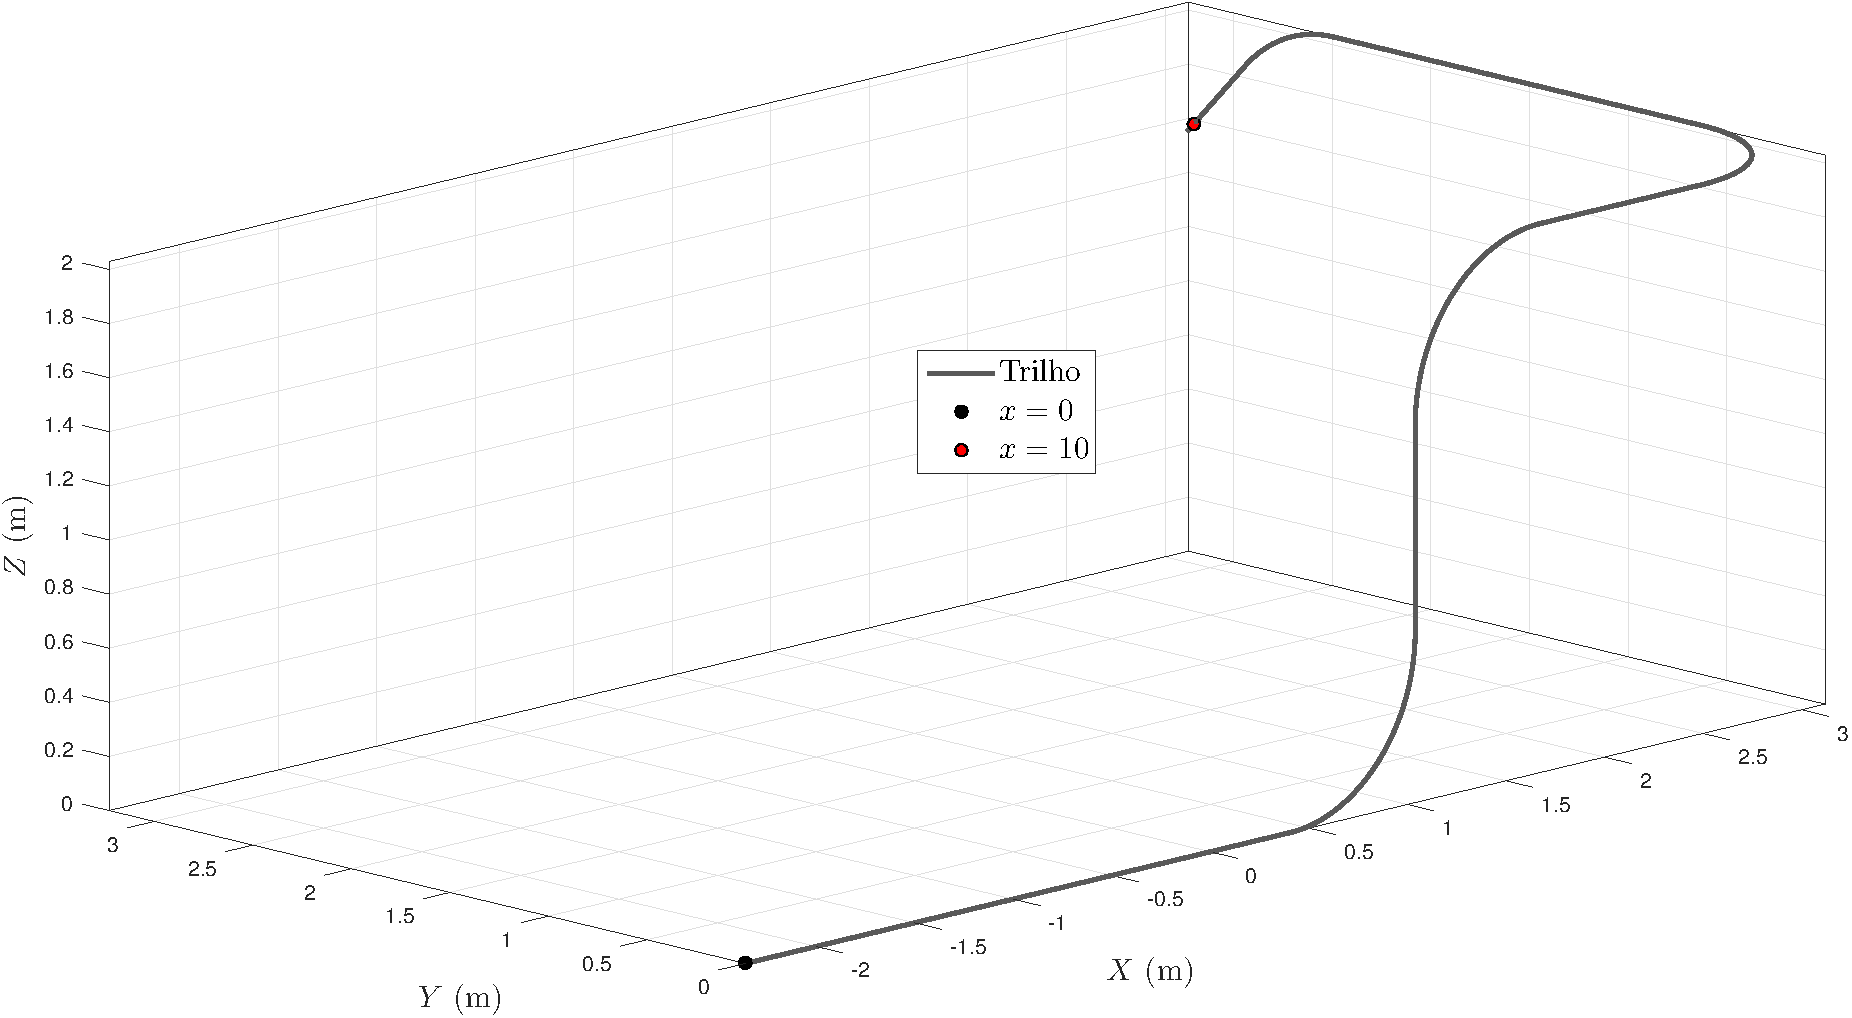
\includegraphics[width=.8\columnwidth]{figs/arqprop/rail_doris.pdf}
\caption{Representa��o gr�fica do mapa alg�brico do trilho at� 10m.}
\label{arqprop/rail_doris.pdf}
\end{figure}

Caso seja inserida uma posi��o alvo maior que o comprimento do trilho, e o
trilho for circular, considera-se uma volta e tira-se a diferen�a, por exemplo
se o trilho posui comprimento 140 e � inserido posi��o alvo 200, considera-se
uma volta e posi��o alvo 60.

\section{Testes da implementa��o da camada Executivo}\label{avaexecutivo}

A avalia��o da camada Executivo � a an�lise e testes por simula��o de suas
responsabilidades dentro dos crit�rios de Arkin. Isto �, como o modo de
implementa��o de cada responsabilidade da camada se comporta em face aos
crit�rios estabelecidos. 

A cria��o de diversos conceitos de processos que s�o executados simultaneamente,
como \textbf{processos reativos vitais, espec�ficos e de recursos dispon�veis},
a decomposi��o de miss�es em tarefas, e a possibilidade de tarefas concorrentes
(\textit{concurrence}), s�o m�todos para cria��o de uma camada com
\textbf{Suporte a paralelismo} e \textbf{Suporte � modularidade}. Al�m disso,
os conceitos criam um m�todo intuitivo para a implementa��o da camada, seguindo
o modelo da naturaza do homem e outros animais, levando a um menor \textbf{Tempo de desenvolvimento}. No entando, paralelismo e modularidade
podem gerar conflitos, os quais devem ser resolvidos por uma fun��o de coordena��o. A
arquitetura h�brida proposta utiliza a subsun��o como fun��o de coordena��o, e
s�o necess�rias avalia��es e testes para verificar sua efici�ncia.

A simula��o consiste na implementa��o dos \textbf{processos reativos}, tarefas
e miss�es simples da DORIS, utilizando a classe implementada
\textbf{SUPPRESSION\_STATE}, apresentada na subse��o~\ref{impexecutivo}, e no
envio de mensagens ROS aos componentes da camada, simulando mensagens do n�vel
Funcional (sa�das de sensores e atuadores do rob�).
Como j� foi discutido, a classe derivada de SMACH � o m�dulo comportamental da
camada Executivo e faz o papel da fun��o de coordena��o por subsun��o. Os
\textbf{processos reativos} e as miss�es da DORIS j� foram documentados na
subse��o~\ref{impexecutivo} e ~\ref{missioncontrol}, respectivamente.


A metodologia de simula��o � composta por tr�s est�gios: 1) Para cada tarefa de
miss�o simples, simular as possibilidades de \textit{outcomes} (resultados das
tarefas), isto �, as ramifica��es de cada tarefa; 2) Simular as intera��es com
os tr�s tipos de \textbf{processos reativos}; e 3) Verificar a finaliza��o da
miss�o, quando todos as tarefas s�o completadas. Abaixo, � demonstrada a
simula��o de uma miss�o simples. O visualizador \textit{smach\_viewer} �
utilizado durante as etapas de simula��o, por disponibilizar os dados dos
estados SMACH em tempo real.

\textbf{Exemplo - simula��o miss�o simples GOTO(80,'fast')}

Ao inicializar o sistema aut�nomo com a miss�o simples \textbf{GOTO(80,'fast')}
(rob� deve se locomover at� a posi��o 80 do trilho, em modo
de velocidade r�pido e pelo menor caminho poss�vel), os \textbf{processos
reativos} s�o executados em paralelo automaticamente. A figura~\ref{proc}
� uma imagem do visualizador \textit{smach\_viewer} que ilustra os processos em
execu��o: em vermelho est� destacada a miss�o simples \textbf{GOTO}; em azul, o
\textbf{processo reativo de recurso dispon�vel}: \textbf{EPOS}, o qual verifica
o status dos motores e drivers EPOS (hardwares); em verde, os \textbf{processos
reativos vitais}: \textbf{Charge}, que verifica o status da bateria, e
\textbf{StateOfTemp}, que verifica a temperatura e umidade do rob�; e em
amarelo, o \textbf{processo reativo espec�fico}: \textbf{OA}
(\textit{ObstacleAvoidance}), que detecta objetos no trilho.

\begin{figure}[!ht]
\centering
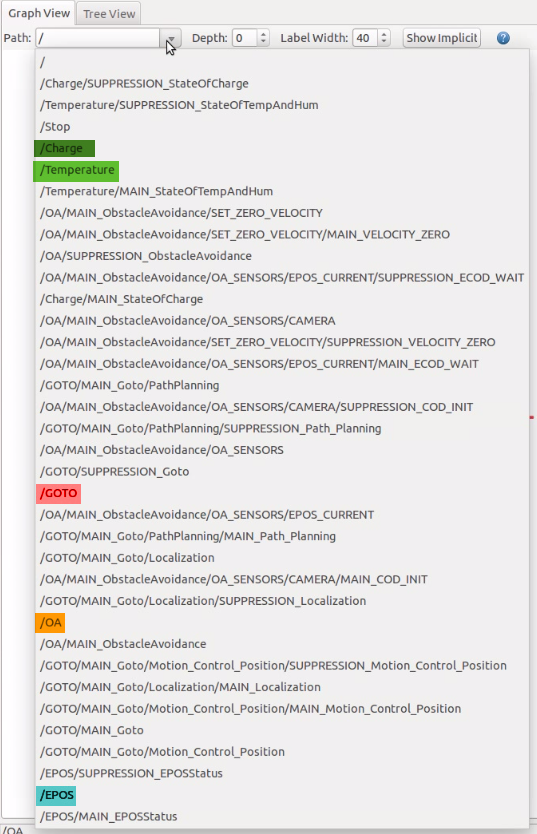
\includegraphics[width=.8\columnwidth]{figs/processos.png}
\caption{Processos em execu��o durante miss�o \textbf{GOTO}.}
\label{proc}
\end{figure}

A tarefa inicial da miss�o simples \textbf{GOTO} � \textbf{Localization}, na
qual permanece at� receber o valor da posi��o do rob� e sua probabilidade.
Caso esta probabilidade esteja dentro do esperado (entre 0.6 e 1), o rob� segue
para a tarefa \textbf{PathPlanning}. A
tarefa \textbf{PathPlanning} requisita o plano de velocidades ao algoritmo
\textbf{MasterPlanning} da camada Funcional. Quando recebido, a
miss�o \textbf{GOTO} segue para sua �ltima tarefa \textbf{Motion\_Control\_Position}.
Esta � um loop que recebe a posi��o do rob�, compara com a tabela recebida do
\textbf{PathPlanning} e envia comando de controle de posi��o ao componente
\textbf{PositionController} da camada Funcional (figura~\ref{maingoto}). 
 
Como a primeira tarefa \textbf{Localization} espera mensagem de ROS da camada
Funcional, uma mensagem ROS com posi��o e probabilidade � enviada pelo terminal
(Ubuntu) ao t�pico \textit{DORIS/Vehicle/Localization}, simulando a camada de
baixo n�vel. Ao receber a mensagem '[30,1]' (posi��o 30 e probabilidade 1), a
tarefa � completada, e a tarefa seguinte, \textbf{PathPlanning}, recebe o dado de posi��o
por \textit{user data} SMACH. \textbf{PathPlanning} envia por mensagem de ROS
comandos ao \textbf{MasterPlanning}, recebe o plano deste e o envia � tarefa
\textbf{Motion\_Control\_Position} tamb�m por \textit{user data} SMACH. 

A figura~\ref{transgoto} mostra as transi��es das tarefas descritas pelo
terminal do Ubuntu onde: em azul, o recebimento da localiza��o e dados da
miss�o (30 � posi��o atual, 80 � posi��o objetivo, 'fast' � o modo de velocidade r�pida);
em verde, a matriz de velocidades e pontos de troca gerados pelo
\textbf{MasterPlanning} da camada Funcional e recebida pela tarefa \textbf{PathPlanning} da miss�o \textbf{GOTO} (camada Executivo); e, em
vermelho, o loop da tarefa \textbf{Motion\_Control\_Position}, a qual recebe
uma localiza��o e controla o rob� por posi��o. Na figura~\ref{transgoto2}, a
mesma transi��o pode ser vista no smach\_viewer, no qual, em verde, s�o as
tarefas em execu��o (no caso, apenas o \textbf{Motion\_Control\_Position}, e o
estado de supress�o).

 De acordo com a metodologia de simula��o, para cada tarefa, devem ser testadas
 os poss�veis \textit{outcomes}. As tarefas \textbf{Localization} e
 \textbf{Motion\_Control\_Position} possuem ramifica��o dependentes de dados da
 camada Funcional: quando \textit{Localization} recebe dados de posi��o
 do rob� com certeza inferior a 60\%, seu \textit{outcome} � o estado
 \textbf{WANDER}, o qual controla o rob� com velocidade 0.1 m/s at� a certeza de
 posi��o aumentar para 60\%; quando \textbf{Motion\_Control\_Position} recebe dados de posi��o com certeza inferior
 a 60\%, seu \textit{outcome} � \textbf{Localization}. Ambas as ramifica��es s�o
 testadas por mensagens de ROS via terminal, por exemplo enviando a mensagem
 '[30,0.4]' (probabilidade 0.4) ao t�pico \textit{DORIS/Vehicle/Localization}, e
 suas transi��es s�o acompanhadas pelo smach\_viewer.

\begin{figure}[!ht]
\centering
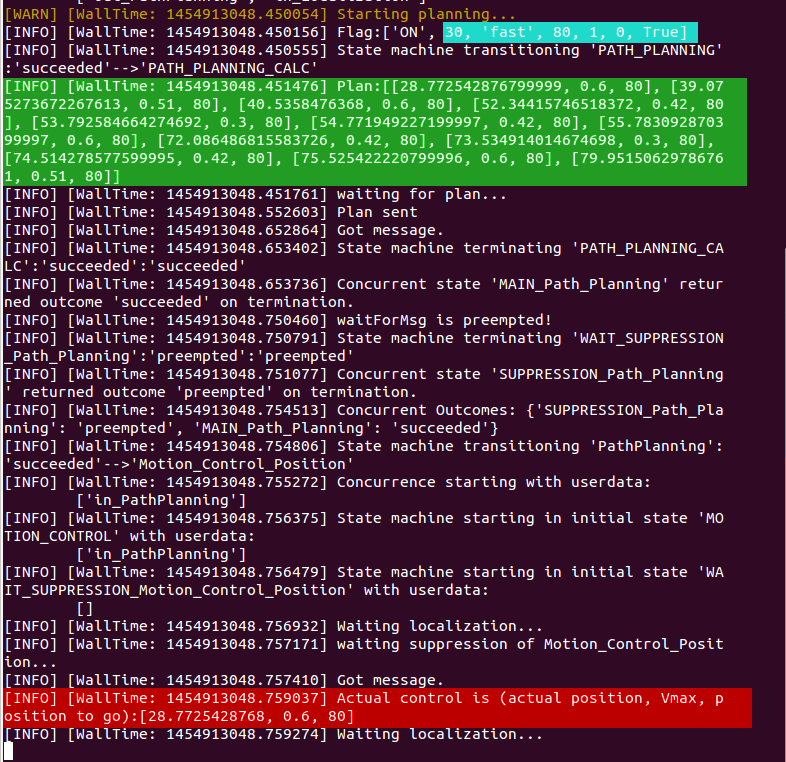
\includegraphics[width=.8\columnwidth]{figs/transitions_goto.png}
\caption{Transi��es da miss�o simples \textbf{GOTO} no terminal.}
\label{transgoto}
\end{figure}

\begin{figure}[!ht]
\centering
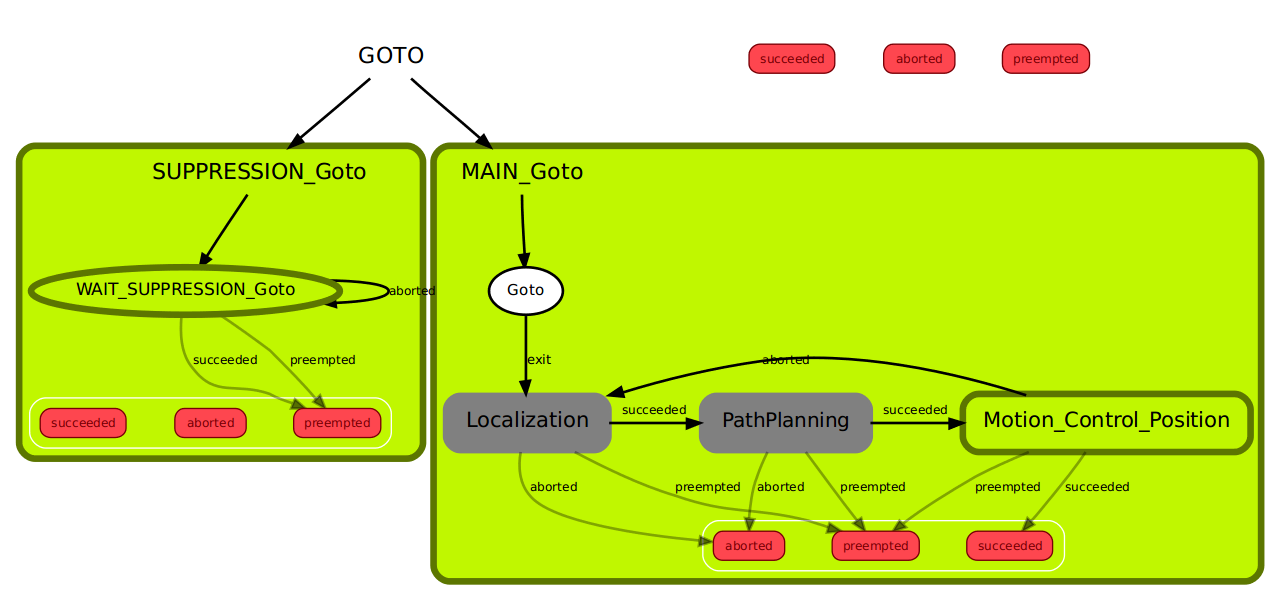
\includegraphics[width=.8\columnwidth]{figs/transition_goto2.png}
\caption{Transi��es da miss�o simples \textbf{GOTO} no smach\_viewer.}
\label{transgoto2}
\end{figure}

A segunda etapa da simula��o s�o as tr�s poss�veis intera��es entre os
tipos de processos reativos. Devem ser observadas as caracter�sticas de
subsun��o: cancelamento de miss�o por processo reativo vital; cancelamento de
miss�o por processo reativo de recurso dispon�vel; e interrup��o de miss�o e
recupera��o de falha por processo reativo espec�fico. 

Exemplo com processo reativo vital: o processo \textbf{Charge} recebe a mensagem
``5'' no t�pico \textit{'DORIS/MCS/StateOfCharge/Status'} (5\% de n�vel de bateria)
e aborta a miss�o \textbf{GOTO} por seguran�a, figura~\ref{abortcharge}
(terminal) e figura~\ref{abortgoto} (smach\_viewer, tarefa em cinza
significa que n�o est� em execu��o).

\begin{figure}[!ht]
\centering
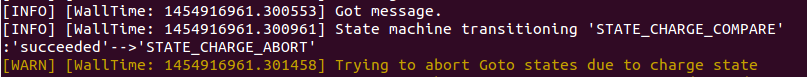
\includegraphics[width=.8\columnwidth]{figs/abortcharge.png}
\caption{Ao receber uma informa��o de n�vel de bateria inferior a 5\%,
\textbf{Charge} aborta a miss�o \textbf{GOTO} (terminal).}
\label{abortcharge}
\end{figure}

\begin{figure}[!ht]
\centering
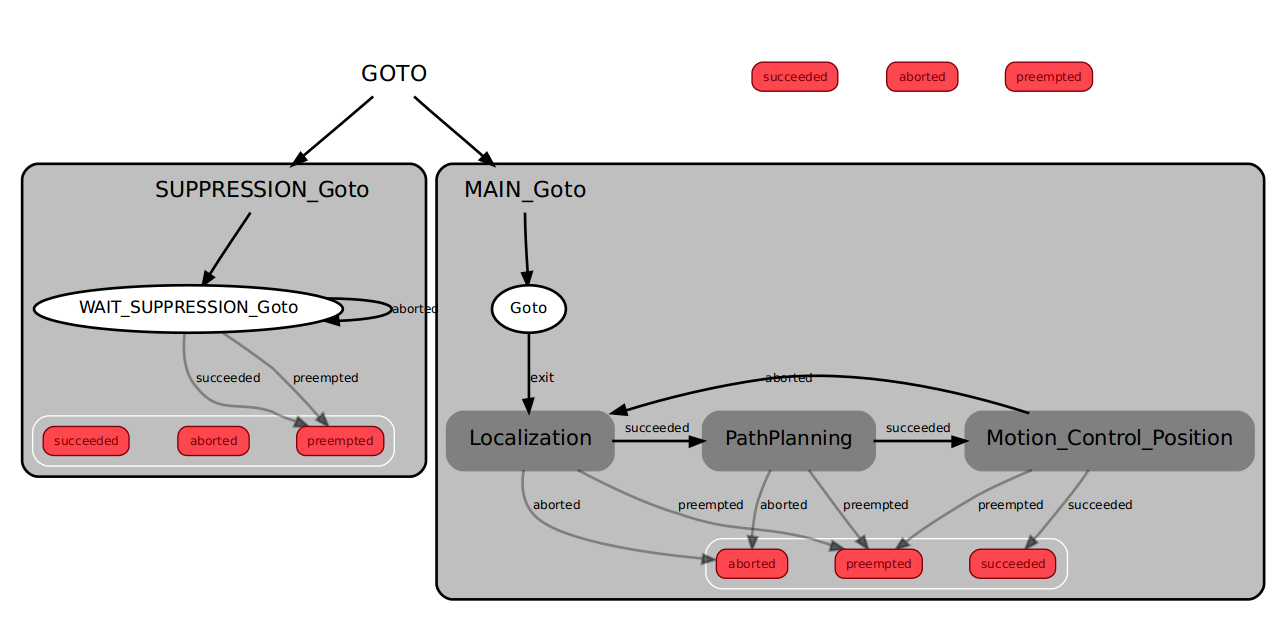
\includegraphics[width=.8\columnwidth]{figs/gotoabort.png}
\caption{Ao receber uma informa��o de n�vel de bateria inferior a 5\%,
\textbf{Charge} aborta a miss�o \textbf{GOTO} (smach\_viewer).}
\label{abortgoto}
\end{figure}

Exemplo com processo reativo de recurso dispon�vel: o processo \textbf{Epos}
recebe a mensagem ``False'' no t�pico \textit{'DORIS/MCS/EPOS/Status'}
(recurso n�o dispon�vel) e aborta a miss�o \textbf{GOTO},
figura~\ref{eposabort} (terminal).

\begin{figure}[!ht]
\centering
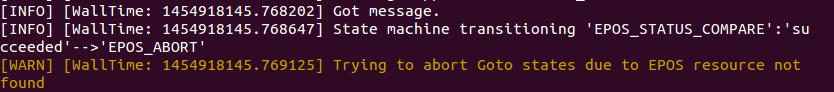
\includegraphics[width=.8\columnwidth]{figs/EPOSabort.png}
\caption{Ao receber uma informa��o de recurso indispon�vel, \textbf{Epos} aborta
a miss�o \textbf{GOTO} (terminal).}
\label{eposabort}
\end{figure}

Exemplo com processo reativo espec�fico: o processo \textbf{OA}
(\textbf{ObstacleAvoidance}) recebe a mensagem ``8'' no t�pico
\textit{'DORIS/Vehicle/EPOS/Current'} (corrente consumida do motor maior que 8
amp�res) e aborta a tarefa \textbf{Motion\_Control\_Position} da miss�o, para um
estado de recupera��o. A miss�o volta � tarefa \textbf{Localiza��o}, o
cart�grafo deve atualizar o mapa do trilho com o obst�culo para rec�lculo da
trajet�ria (sentido contr�rio).

Dessa forma, as responsabilidades \textbf{Sequenciador} e \textbf{Selecionador}
da camada Executivo atendem aos crit�rios \textbf{Suporte a paralelismo},
\textbf{Suporte � modularidade} e \textbf{Tempo de desenvolvimento}, utilizando
a metodologia de simula��o adotada. Al�m disso, o \textbf{Desempenho em executar
tarefas} � aumentado com o paralelismo e a modelagem seguindo a metodologia e
conceitos de processos estabelecidos. A \textbf{Robustez} � alcan�ada pelas
ramifica��es das tarefas, pelos processos reativos, e est� contida
na responsabilidade de recupera��o de falhas. A modelagem das tarefas n�o pode
ser realizada em tempo de execu��o, o que n�o � desvantagem, pois a metodologia
de simula��o deve ser seguida e sistemas aut�nomos n�o devem ser executados
sem testes pr�vios. A \textbf{Flexibilidade em tempo de execu��o} deve estar
dispon�vel na camada Funcional, mas n�o na camada aut�noma.

Por fim, o \textbf{\textit{Niche targetability}} � muito abrangente, j� que
a camada comporta rob�s modelados por tarefas sequenciais e processos reativos
paralelos, o mecanismo mais comum encontrado na natureza. 

\section{Testes da implementa��o da camada Planejador}\label{avaplanejador}

Assim como a camada Executivo, os testes da camada Planejador � a avalia��o das
responsabilidades desenvolvidas para a camada no contexto dos crit�rios de
Arkin, ou seja, � a an�lise de \textbf{controle de miss�o},
\textbf{agendador} e \textbf{cart�grafo} em face aos crit�rios.

As defini��es de tipos de miss�es, simples, complexas e desconhecidas,
introduzidas na subse��o~\ref{missioncontrol}, mostram a decomposi��o
estabelecida, e estimulam uma implementa��o em m�dulos na camada Planejador.
O \textbf{controle de miss�o} traduz as miss�es complexas, isto �,
decomp�e as miss�es complexas em miss�es simples, de maneira sequencial ou paralela,
provendo o \textbf{Suporte � modularidade} e \textbf{Suporte ao paralelismo}.

Na classe miss�o, tr�s m�todos devem ser implementados: $mission(arguments)$,
onde as tarefas da miss�o s�o implementadas sequencialmente, pertencente �
camada Executivo; $reactives(arguments)$, onde s�o definidos os
\textit{processos reativos espec�ficos} da miss�o, tamb�m pertencente � camada
Executivo; e $execute(arguments)$, onde o m�todo $mission(arguments)$ �
executado, junto com as miss�es simples que comp�e a miss�o, paralela ou
sequencialmente. A organiza��o cria uma ferramenta para implementa��o de
miss�es, agilizando o \textbf{Tempo de desenvolvimento}. Al�m disso, a flexibilidade na modelagem das miss�es complexas e o paralelismo permitem a
otimiza��o do \textbf{Desempenho em executar tarefas}, sem comprometer a camada Executivo.

A \textbf{Robustez} da arquitetura pertence � camada Executivo, nas ramifica��es
dos \textit{outcomes}, e aos \textbf{Agendador} e \textbf{controle de
miss�o}, na camada Planejador: erros nas miss�es agendadas devem ser
reprogramadas para o futuro; e o feedback ao usu�rio dispon�vel pelo
\textbf{controle de miss�o} � uma inform��o
que pode ser interpretada e utilizada para algumas tomadas de decis�o. 


O \textbf{\textit{Niche targetability}} � garantido pela flexibilidade na
implementa��o das miss�es complexas do \textbf{controle de miss�o}, e a
diversidade do \textbf{cart�grafo}, o qual pode gerar diversos modelos de mundo pelos os algoritmos da camada
Funcional.

Como a camada Executivo, a \textbf{Flexibilidade em tempo de execu��o} �
comprometida propositalmente para simula��es serem exaustivamente avaliadas
antes da execu��o do sistema aut�nomo no rob�.

\textbf{Exemplo - simula��o miss�o complexa INSPECTION(['VIDEO'],[80,'fast'])}

Na simula��o da camada Planejador, � avaliado apenas o \textbf{controle de
miss�o}, pois, apesar de as outras responsabilidades terem sido discutidas
previamento e seu funcionamento interno detalhado, elas n�o foram totalmente
implementadas e integradas � arquitetura.

As etapas da simula��o s�o: requisi��o de miss�o complexa pelo usu�rio; tradu��o
da miss�o complexa; execu��o da miss�o; feedback ao usu�rio. A interface
gr�fica de usu�rio n�o est� finalizada, mas as mensagens de usu�rio podem ser
simuladas por mensagens ROS via terminal.

Na camada Planejador, h� tr�s \textit{threads} esperando mensagens de ROS da
interface de usu�rio: 1) \textit{thread} que aguarda a mensagem da miss�o; 2)
\textit{thread} que espera o comando ``Play'', o qual d� in�cio a execu��o; e
3) \textit{thread} $\textbf{STOP}$, que finaliza a execu��o, isto �, aborta o
sistema aut�nomo (todas as suas miss�es e processos). Para o exemplo de miss�o
complexa $\textbf{INSPECTION}$, s�o enviadas as mensagens: 1)
'[[1,[0],['slow',80,1,0,True]]]' ao t�pico \textit{'DORIS/MCS/Mission'}
(mensagem de miss�o complexa, onde 1 representa a miss�o $\textbf{INSPECTION}$,
[0] representa inspe��o por v�deo, e ['slow',80,1,0,True] s�o os par�metros
da miss�o simples $\textbf{GOTO}$); 2) ``Play'' ao t�pico
\textit{'DORIS/MCS'}, inicializando a execu��o do sistema aut�nomo.

O  \textbf{controle de miss�o} chama o m�todo $execute(arguments)$ da miss�o
complexa \textbf{INSPECTION}, o qual a decomp�e, como pode ser visto na
figura~\ref{executeinspection}. Na figura, temos: 
\begin{itemize}
  \item Em verde, primeiramente, � executada a miss�o principal
  \textbf{INSPECTION\_INIT}, composta por uma tarefa (m�dulo
  \textbf{SUPPRESSION}), cujo \textbf{SUPPRESSION\_MAIN} aguarda a finaliza��o
  da miss�o, isto �, fim da miss�o \textbf{INSPECTION}. Esta miss�o principal �
  necess�ria, pois ela que ``segura'' a execu��o de toda a miss�o complexa,
  podendo cancel�-la por completo, se requisitada;
  \item Em azul, logo em seguida, � executada a miss�o simples \textbf{DETECT},
  que inicializa o algoritmo de detec��o de anomalias. � uma miss�o em paralelo,
  pois ela � executada at� o fim da miss�o complexa;
  \item Em vermelho, est�o representadas as miss�es simples sequenciais.
  ``join()'' em um \textit{thread} significa que uma miss�o simples est� sendo
  executada em uma nova \textit{thread}, mas a \textit{thread} principal
  (miss�o complexa) s� prossegue ap�s a finaliza��o da miss�o simples, o que mostra o car�ter sequencial. As miss�es simples sequenciais
  s�o: $\textbf{GOTO(80,'slow')}$, $\textbf{StopDETECT}$ e
  $\textbf{StopINSPECTION}$. A miss�o simples $\textbf{StopINSPECTION}$ deve
  existir, pois finaliza a miss�o simples principal \textbf{INSPECTION\_INIT}.
  \item Como n�o h� processos reativos espec�ficos, n�o h� comando de
  finaliza��o destes.
\end{itemize}
 

\begin{figure}[!ht]
\centering
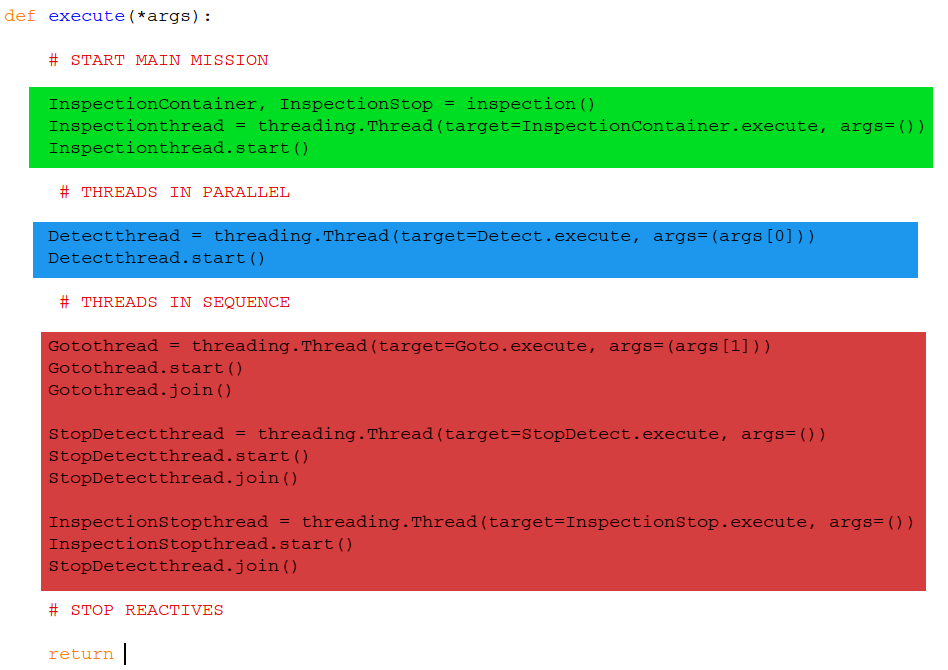
\includegraphics[width=1\columnwidth]{figs/executeinspection.png}
\caption{M�todo $execute$ da miss�o \textbf{INSPECTION}.}
\label{executeinspection}
\end{figure}

Essa metodologia deve ser seguida em todas as implementa��es de miss�es
complexas e, futuramente, em miss�es desconhecidas. A an�lise da simula��o
(execu��o da miss�o complexa) se torna, ent�o, equivalente � an�lise da execu��o
das miss�es simples que a comp�e, e pode ser realizada pelo smach\_viewer. A
figura~\ref{inspectionfull} mostra as miss�es simples e processos reativos em
execu��o, quando a miss�o complexa \textbf{INSPECTION} � inicializada. Segue a
legenda de cores:
\begin{itemize}
  \item Em vermelho, est�o destacadas as miss�es simples: \textbf{GOTO}
  (sequencial) e \textbf{DETECT} (paralela);
  \item Em azul, o \textbf{processo reativo de recurso dispon�vel}:
  \textbf{EPOS}, o qual verifica o status dos motores e drivers EPOS
  (hardwares). Observe que h� a necessidade de implementa��o de outro
  \textbf{processo reativo de recurso espec�fico}: \textbf{CAMERA}, que verific�
  o status da c�mera e pode abortar a miss�o \textbf{DETECT} e
  \textbf{INSPECTION} caso o recurso n�o seja detectado;
  \item Em verde, os \textbf{processos reativos vitais}: \textbf{Charge}, que
  verifica o status da bateria, e \textbf{StateOfTemp}, que verifica a temperatura e umidade do rob�;
   \item Em amarelo, o \textbf{processo reativo espec�fico} da miss�o simples
   \textbf{GOTO}: \textbf{OA} (\textit{ObstacleAvoidance}), que detecta
   objetos no trilho. Neste exemplo, as outras miss�es simples n�o possuem
   \textbf{processos reativos espec�ficos}, caso tivessem, estes seriam
   executados sequencialmente, juntos �s miss�es.
\end{itemize}

\begin{figure}[!ht]
\centering
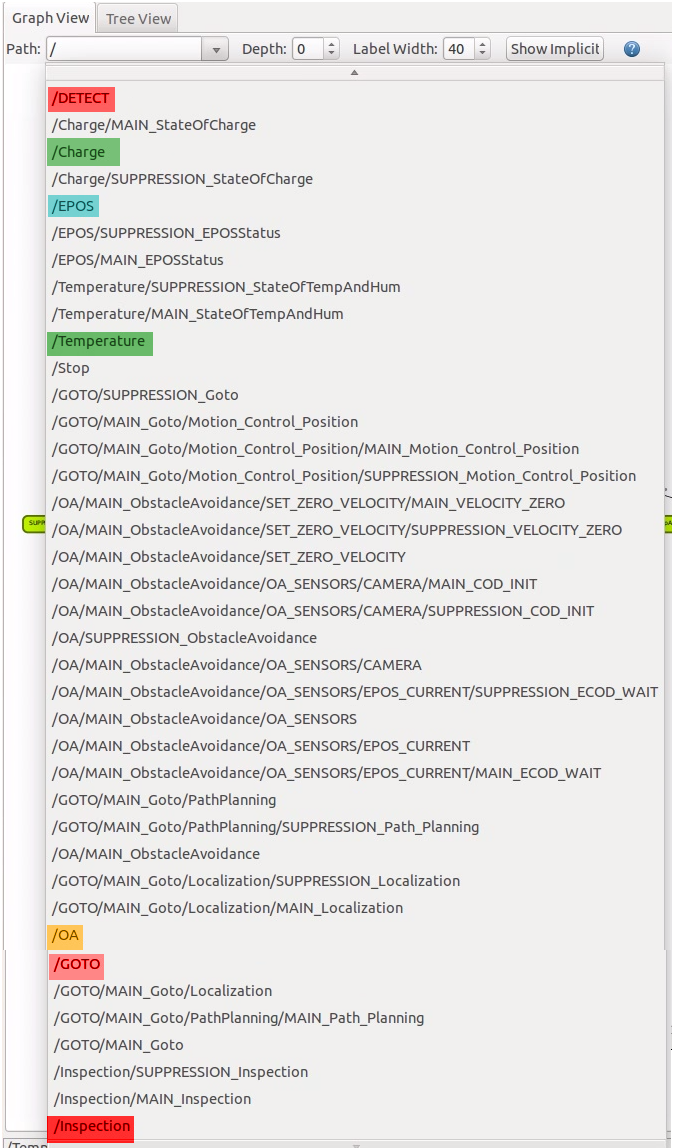
\includegraphics[width=.8\columnwidth]{figs/inspectionfull.png}
\caption{Miss�es e processos na execu��o da miss�o complexa \textbf{INSPECTION}.}
\label{inspectionfull}
\end{figure}

%TODO Falar de metodo que da feedback da porcentagem da missao
  \chapter{Conclus�es e trabalhos futuros}\label{conclusao}

A disserta��o ``Arquitetura h�brida de um rob� m�vel guiado por
  trilhos'' foi dividia em tr�s partes principais: revis�o bibliogr�fica,
arquitetura proposta, e resultados.

A revis�o bibliogr�fica, cap�tulo~\ref{bibliografia}, apresentou os conceitos
b�sicos (se��o~\ref{conceitos}) para o entendimento da disserta��o, de acordo
com os principais roboticistas. � realizada uma revis�o detalhada e
cronol�gica dos paradigmas da rob�tica e suas principais arquiteturas: deliberativa, reativa, e h�brida, comentando
vantagens, desvantagens e mostrando aplica��es em rob�s pioneiros, de transi��o
e atuais. A an�lise das arquiteturas conclui que a arquitetura h�brida de tr�s
camadas � aquela com o maior n�mero de aplica��es complexas e bem sucedidas e
que deve ser explorada para o rob� de estudo, DORIS. Por fim, a revis�o
bibliogr�fica explora os diferentes ambientes de desenvolvimento de software em rob�tica (RDEs), apresentando vantagens e
desvantagens dos principais e mais utilizados na literatura. Uma avalia��o
competitiva mostrou que ROS e SMACH s�o ferramentas excelentes para as camadas
Funcional e Executivo, respectivamente, e foram exploradas na solu��o proposta pelo autor.

A arquitetura proposta, cap�tulo~\ref{arquipro}, � a aplica��o do conhecimento
adquirido e o que foi discutido durante a revis�o bibliogr�fica, tentando aproveitar as vantagens da fus�o de arquiteturas
deliberativas e reativas, e contornando suas desvantagens. Na arquitetura
h�brida de tr�s camadas, h� variadas formas de implementa��o das camadas e suas
responsabilidades. O cap�tulo � dividido na implementa��o dessas camadas,
destacando e compilando suas responsabilidades. Tamb�m s�o definidos novos
conceitos para garantir modularidade e flexibilidade da solu��o, como plano de miss�o, miss�o
simples, miss�o complexa, tarefas, e processos reativos.

A camada Planejador � implementada com as responsabilidades controle de miss�o,
agendador e cart�grafo. A primeira � uma interface usu�rio-rob� que traduz os
comandos e miss�es do n�vel superior ao n�vel Executivo, e exibe o feedback
das miss�es ao operador. O agendador memoriza o plano de miss�o dentro do rob�,
marca um hor�rio para execu��o, e possui um algoritmo de recupera��o de falhas
para reagendar o plano. O cart�grafo � uma compila��o de mapas, gerencia os
modelos do mundo, cria novos modelos para otimizar as tarefas, e os
mant�m atualizados com a ajuda da camada Funcional.

A camada Executivo usa SMACH como ferramenta para modelagem de tarefas do rob�,
e organiza a implementa��o nas responsabilidades sequenciador, selecionador,
monitoramento e recupera��o de erros, e gerenciamento de recursos, de forma a
garantir modularidade, flexibilidade, facilidade de implementa��o e desempenho
de execu��o. Al�m disso, � desenvolvida uma arquitetura de subsun��o, na camada, 
com a ferramenta SMACH e ROS, obtendo assim as vantagens da fun��o de coordena��o competitiva
para tarefas conflitantes. As desvantagens da subsun��o, como
\textit{situatedness} e escalabilidade, s�o contornadas a partir de uma
delibera��o na camada.

A camada Funcional utiliza ROS como \textit{framework} e comunica��o entre
componentes. Os componentes foram desenvolvidos em m�dulos e na forma
recomendada pelos desenvolvedores de ROS e CLARAty, estado da arte na
implementa��o Funcional. � um software orientado a objeto, obtendo assim modularidade de
hardware, e estrutura��o apropriada de software para usar as propriedades de
heran�a. Nesta camada, ainda � desenvolvido o algoritmo de planejamento de
trajet�ria e velocidades (\textit{Motion Planning}). 

Ao fim do detalhamento da implementa��o, o documento segue para os resultados da
arquitetura, onde DORIS � o estudo de caso. Novamente,
dada a modularidade da solu��o, os testes das camadas podem ser realizados
independentemente e, portanto, o cap�tulo~\ref{result} foi dividido pelas
camadas. Uma metodologia de testes
foi proposta e as camadas s�o avaliadas pelos crit�rios sugeridos por Arkin.

A avalia��o de resultados da camada Funcional s�o testes exaustivos de
componentes com os hardwares do rob�. Drivers de sensores, atuadores e
algoritmos s�o testados, e o rob� pode ser teleoperado com joystick ou por
interface web. O reposit�rio ROS e a organiza��o de um software orientado
a objeto aumentam a facilidade de implementa��o e passam por todos os
crit�rios de Arkin com excel�ncia.

A avalia��o da camada Executivo � a simula��o e avalia��o das miss�es simples e
tarefas modeladas, da arquitetura de subsun��o implementada, e das desvantagens
contornadas. Todas as responsabilidades da camada foram avaliadas e inseridas
nos crit�rios de Arkin. Uma miss�o simples foi decomposta, detalhada e analisada
nesta etapa, utilizando a metodologia proposta. Al�m disso, a ferramenta SMACH e
o visualizador smach\_viewer foram importantes para a solu��o, garantindo o paralelismo e a modularidade.

Por fim, a camada Planejador foi avaliada perante os crit�rios de Arkin. A
metodologia imposta na implementa��o da camada e a organiza��o,
cria��o e defini��o de novos conceitos de miss�es, garantiram modularidade,
paralelismo e flexibilidade da solu��o. Os testes mostraram o sistema aut�nomo
integrado e em funcionamento.

Dessa forma, a disserta��o � um estudo profundo no tema de arquiteturas
rob�ticas e a tentativa de compilar ideias, criar novos conceitos e propor uma arquitetura
h�brida mais geral para rob�s aut�nomos na aplica��o de inspe��o, e que possuem
desafios semelhantes � DORIS, isto �, AUVs e UGVs. A arquitetura se inspira na
natureza, no funcionamento do corpo humano e de outros animais, para criar uma
metodologia intuitiva de implementa��o e avalia��o.

\section{Trabalhos futuros}

Os trabalhos futuros se referem �s responsabilidades n�o finalizadas para cada
camada da arquitetura h�brida proposta, � integra��o das
camadas no rob�, isto �, incluir o sistema aut�nomo no rob� (sair do ambiente
confort�vel da simula��o), � realiza��o de testes em outros sistemas rob�ticos
(como novos desafios de planejamento de trajet�rias), e � formaliza��o
matem�tica das tarefas.

Na camada Funcional, s�o necess�rias implementa��es de algoritos SLAM para o
cart�grafo da camada Planejador, a integra��o dos diversos algoritmos de
detec��o de anomalias, o algoritmo de localiza��o, e controle do manipulador.

Na camada Executivo, � necess�ria a modelagem de miss�es e tarefas em rela��o ao
manipulador do rob� e outras funcionalidades simples. A camada Executivo j�
possui todas as responsabilidades finalizadas e simuladas, de forma que apenas
alguns ajustes e modelagem de novas funcionalidades s�o necess�rias.

Na camada Planejador, � necess�rio desenvolver a interface gr�fica de usu�rio, e
finalizar as responsabilidades de agendador e cart�grafo. O cart�grafo depende
da camada Funcional e deve ser implementada concomitantemente. O agendador n�o �
essencial para o sistema aut�nomo, mas importante para um rob� de inspe��o e
outras aplica��es, logo � necess�ria para uma arquitetura mais geral.

A implementa��o de tarefas com a ferramenta SMACH n�o possui formalismo
matem�tico, logo n�o h� an�lise de conflitos, deadlocks e avalia��o das
m�quinas de estados. As FSMs SMACH n�o possuem modelagem igual � FSM
padr�o, logo a teoria de FSM n�o pode ser aplicada. H� a necessidade do
desenvolvimento de um modelo matem�tico, de forma que o sistema n�o fique
dependente de exaustivas simula��es.

Por fim, s�o necess�rios testes da arquitetura em outros rob�s, a fim de testar
o crit�rio \textit{niche targetability} de Arkin.


  \backmatter
  \nocite{*}
  \bibliographystyle{coppe-unsrt}
  \label{initbib}
  \bibliography{thesis}
  \label{endbib} 
  \appendix
  %\chapter{C�digo Fonte}

\end{document}
